\documentclass[12pt]{article}
\usepackage[utf8]{inputenc}
\usepackage[T1]{fontenc}
\usepackage{geometry}
\usepackage{graphicx}
\usepackage{makeidx}
\geometry{margin=2.5cm}
\usepackage{fancyhdr}

\begin{document}
	
	\thispagestyle{empty}
	
	\begin{center}
		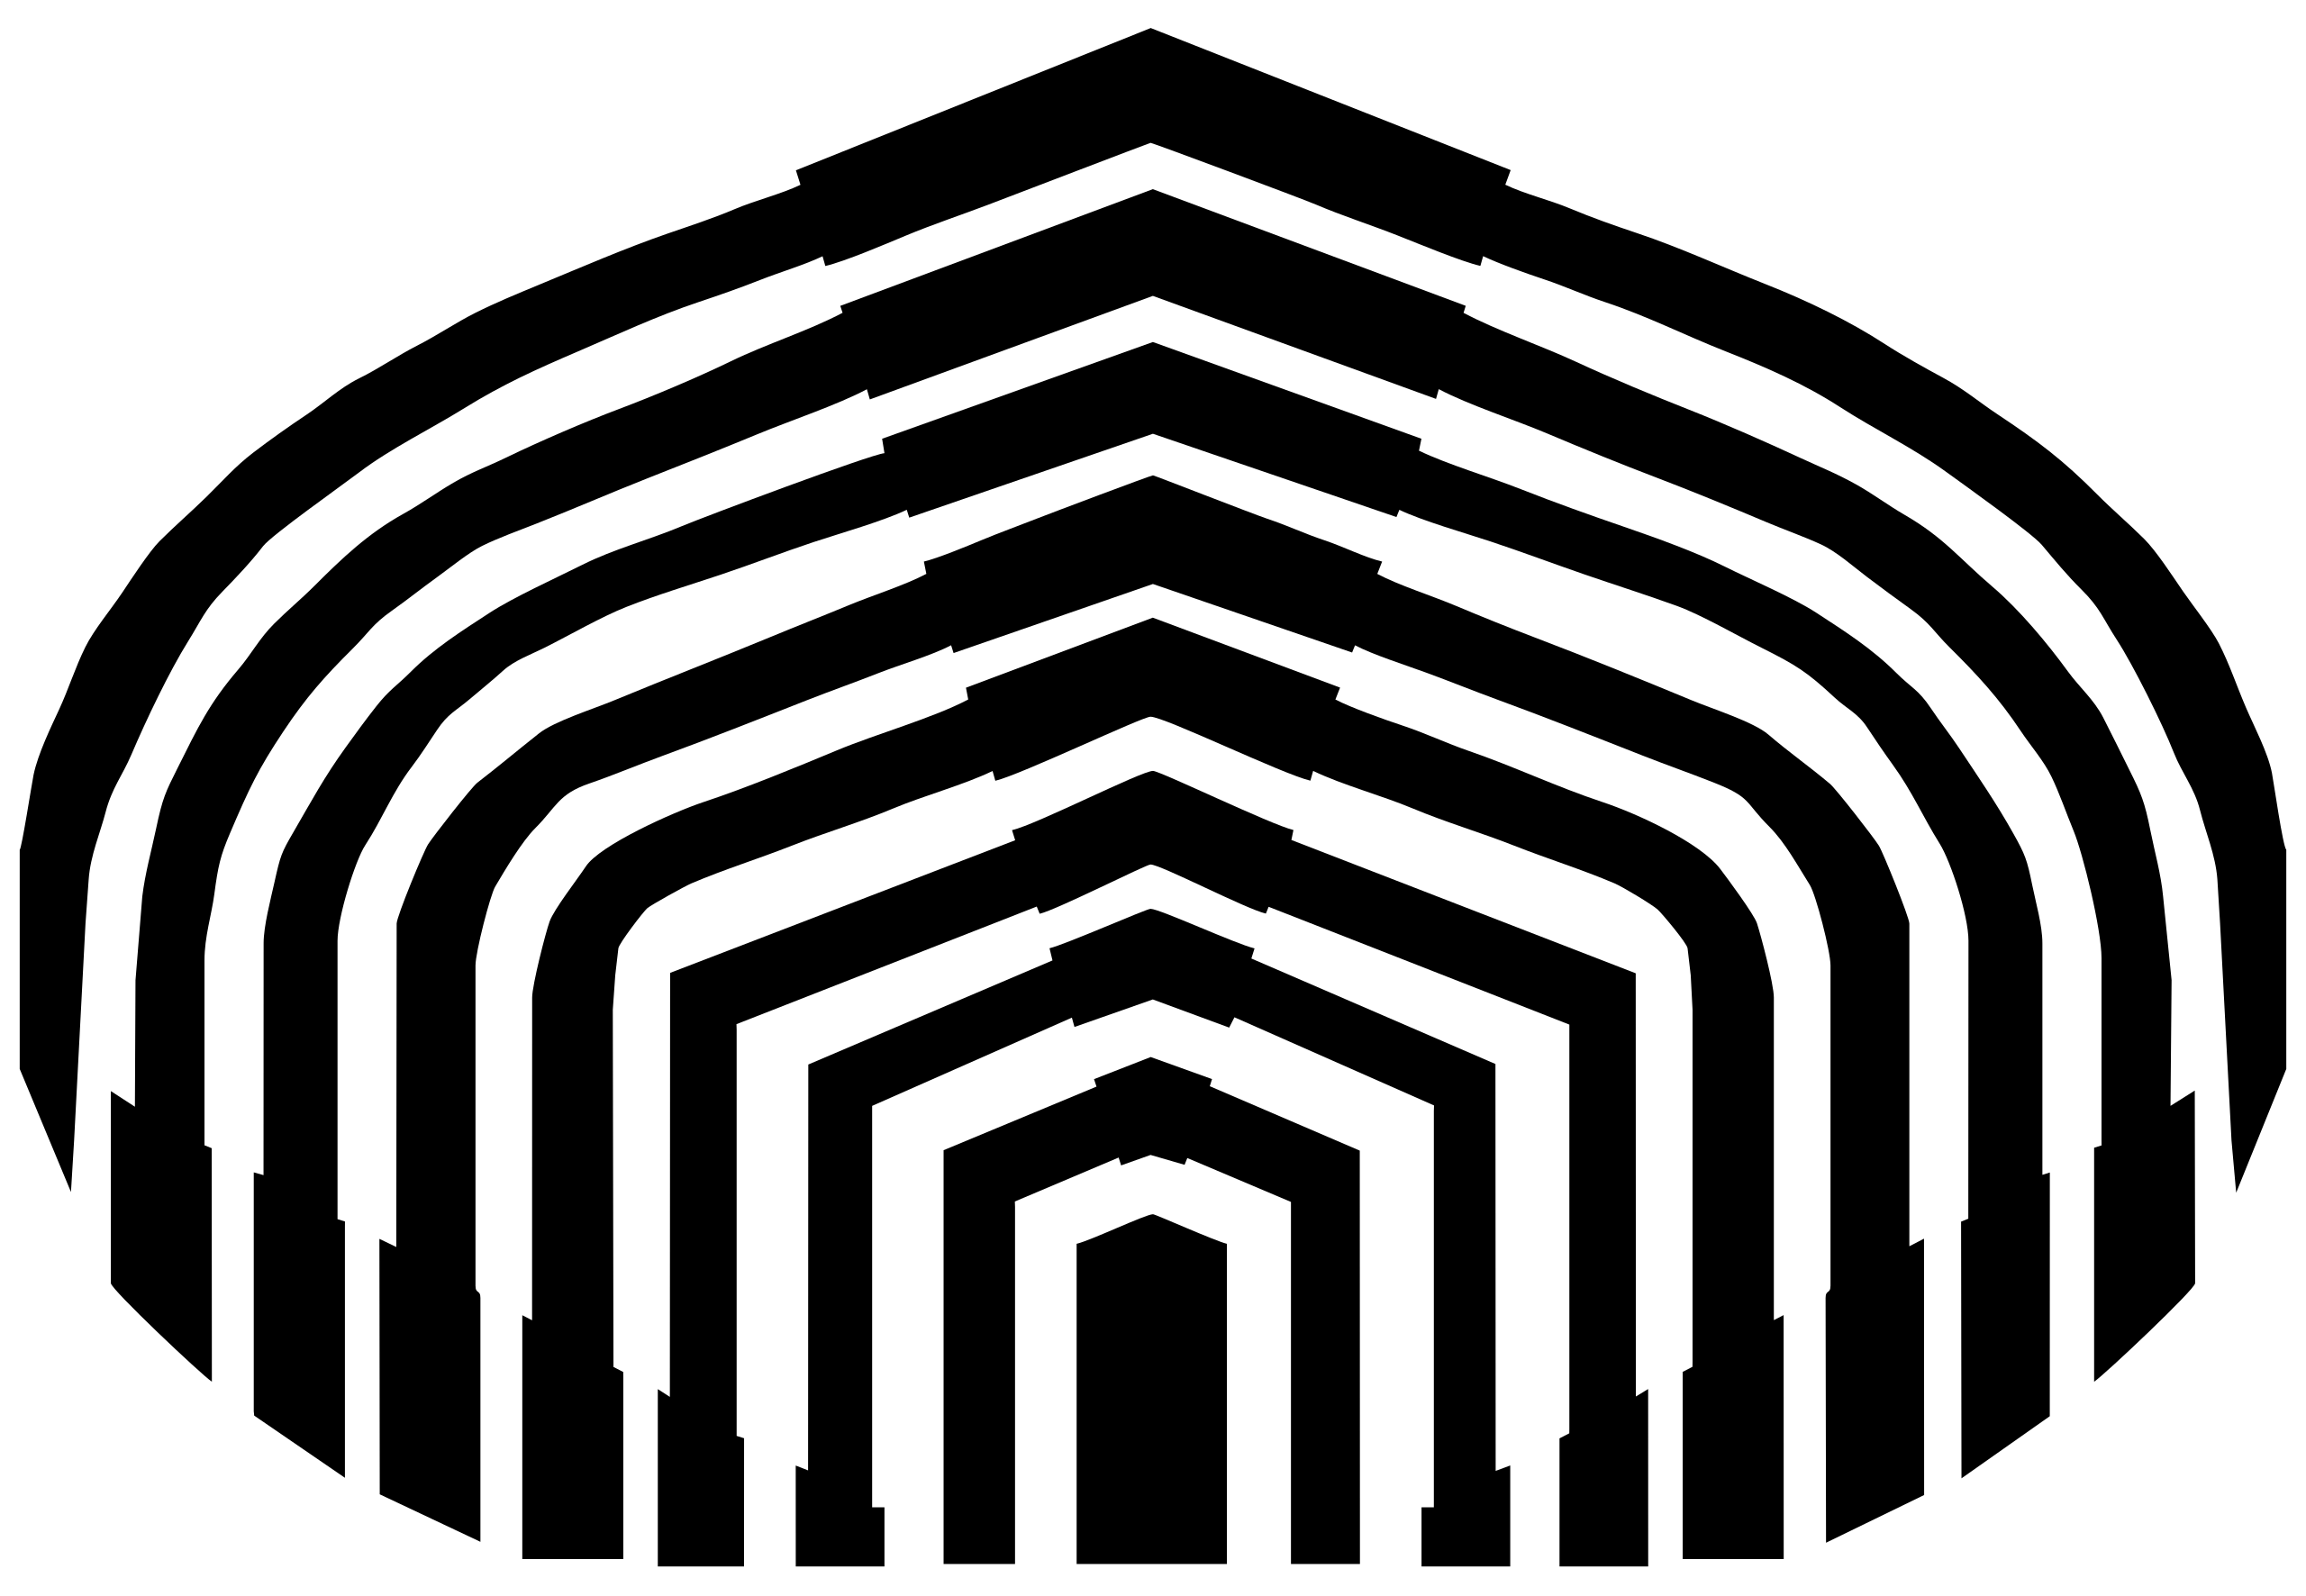
\includegraphics[width=3.1cm,height=2cm]{logo}\\
		UNIVERSIDAD SIMÓN BOLÍVAR\\
		DEPARTAMENTO DE ELECTRÓNICA Y CIRCUITOS\\
		EC1281 - LABORATORIO DE MEDICIONES ELÉCTRICAS\\
		SECCIÓN 1 - GRUPO 1\\
		
		\vspace{7cm}
		\textbf{\Large INFORME - PRÁCTICA \#5}\\
		PRESENTACIÓN X-Y MEDICIONES CON EL OSCILOSCOPIO SOBRE CIRCUITOS RC Y RL\\
	\end{center}
	
	\begin{flushleft}
		\vspace{8cm}
		\hfill Integrantes:\\
		\hfill {\large Luis Becerra - 1910557}\\
		\hfill {\large Lorena Rojas - 1910469}\\
	\end{flushleft}
	
	\newpage
	
	\pagenumbering{Roman}
        \setcounter{page}{2}
	
	\begin{center}
		\textbf{\large RESUMEN}\\
	\end{center}
	
		En esta práctica, se exploró el funcionamiento y las técnicas de medición del osciloscopio. Los objetivos incluyeron el análisis de las características corriente-voltaje de elementos lineales y no lineales, así como la medición de frecuencias y desfasajes utilizando la presentación X-Y. Se llevaron a cabo diversos experimentos, montando circuitos y realizando mediciones con el osciloscopio. Se determinaron las características corriente-voltaje de una resistencia desconocida y un diodo zener, tanto en el dominio del tiempo como en la presentación XY. Además, se realizaron mediciones de desfasajes en circuitos con capacitores e inductores. Las figuras de Lissajous se utilizaron para medir la frecuencia de la línea. Se registraron las mediciones y se tomaron fotografías de las formas de onda y las gráficas obtenidas. En conclusión, la práctica permitió profundizar en el conocimiento del osciloscopio y aplicar técnicas de medición en diversos circuitos.
	
	\newpage
	
	\begin{center}
		\textbf{\large ÍNDICE}\\
	\end{center}
	
	\noindent \textbf{RESUMEN} \hfill \textbf{II}\\
	\noindent \textbf{ÍNDICE} \hfill \textbf{III}\\
	\noindent \textbf{MARCO TEÓRICO} \hfill \textbf{1}\\
	\noindent \textbf{METEDOLOGÍA} \hfill \textbf{}\\
	\noindent \textbf{RESULTADOS} \hfill \textbf{}\\
	\noindent \textbf{ANÁLISIS DE RESULTADOS} \hfill \textbf{}\\
	\noindent \textbf{CONCLUSIONES} \hfill \textbf{}\\
	\noindent \textbf{BIBLIOGRAFÍA} \hfill \textbf{}\\
	\noindent \textbf{ANEXOS} \hfill \textbf{16}\\
	
	\newpage
	
	\pagenumbering{arabic}
	
	\begin{center}
		\textbf{\large MARCO TEÓRICO}\\
	\end{center}
		
	\textbf{1. Modalidad XY del osciloscopio}\\
	
	El osciloscopio es un instrumento ampliamente utilizado en el ámbito de la electrónica y las telecomunicaciones para visualizar y medir señales eléctricas. En su modalidad XY (eje X e Y), el osciloscopio permite representar gráficamente la relación entre dos señales en un plano cartesiano, lo cual resulta especialmente útil para analizar las características corriente-voltaje de elementos lineales y no lineales, así como para medir frecuencias y desfasajes utilizando las Figuras de Lissajous.\\
	
	En la modalidad XY, el osciloscopio se utiliza en combinación con un generador de funciones que suministra una señal de voltaje de referencia y un circuito bajo prueba que genera una señal de corriente o voltaje. Estas señales se conectan a los canales X e Y del osciloscopio, respectivamente, y se representan en el plano XY, donde el eje X representa una señal y el eje Y representa la otra señal.\\
	
	
	
	\textbf{2. Características corriente-voltaje de elementos lineales}\\
	
	\begin{itemize}
		\item \textbf{Definición de características corriente-voltaje}
		
		Las características corriente-voltaje, también conocidas como curvas I-V o curvas de transferencia, describen la relación entre la corriente eléctrica que fluye a través de un componente o circuito y la tensión aplicada a dicho componente. Estas características son representativas del comportamiento eléctrico de los elementos y proporcionan información crucial sobre su funcionamiento.
		
		\item \textbf{Medición de la característica corriente-voltaje en elementos lineales}
		
		La medición de la característica corriente-voltaje en elementos lineales se realiza mediante la configuración de un circuito de medición adecuado. El objetivo es aplicar diferentes niveles de tensión al elemento lineal y medir la corriente resultante para obtener los puntos necesarios para trazar la curva I-V.
		
		\item \textbf{Configuración del circuito de medición}
		
		Para medir la característica corriente-voltaje en un elemento lineal, se debe construir un circuito adecuado que permita aplicar una tensión variable y medir la corriente correspondiente. La configuración más común implica el uso de una fuente de tensión en serie con el elemento lineal y un amperímetro en serie para medir la corriente.\\
		
		La fuente de tensión proporciona la tensión de entrada variable, que se aplica al elemento lineal. El amperímetro se coloca en serie para medir la corriente que fluye a través del elemento. Se debe asegurar que el amperímetro tenga una resistencia interna baja para evitar perturbaciones significativas en el circuito y obtener mediciones precisas.\\
		
		Al variar la tensión de entrada y medir la corriente resultante, se pueden obtener varios puntos en la curva I-V. Estos puntos se pueden graficar para visualizar la relación entre la corriente y la tensión y analizar el comportamiento lineal del elemento. 
	\end{itemize}
	
	\textbf{3. Características corriente-voltaje de elementos no lineales}
	
	\begin{itemize}
		\item \textbf{Comportamiento no lineal de los elementos}
		
		A diferencia de los elementos lineales, los elementos no lineales exhiben un comportamiento no proporcional entre la corriente y la tensión aplicada. En otras palabras, la relación entre la corriente y la tensión no sigue una ley lineal, sino que puede ser no lineal y presentar efectos no despreciables, como la distorsión armónica, la rectificación, la conmutación o la generación de armónicos.\\
		
		El comportamiento no lineal puede ser causado por diversas razones, como la dependencia de la temperatura, la presencia de elementos activos (como transistores o diodos) o la interacción con campos eléctricos o magnéticos. Estos elementos no lineales requieren un análisis específico y una comprensión detallada de sus características corriente-voltaje.
		
		\item \textbf{Medición de la característica corriente-voltaje en elementos no lineales}
		
		La medición de la característica corriente-voltaje en elementos no lineales también implica la configuración de un circuito de medición adecuado. Sin embargo, debido al comportamiento no lineal de estos elementos, se requieren enfoques diferentes para obtener una representación precisa de su curva I-V.
		
		\item \textbf{Configuración del circuito de medición}
		
		La configuración del circuito de medición para elementos no lineales puede variar según el tipo de elemento y su comportamiento específico. En general, se puede utilizar una fuente de tensión variable en serie con el elemento no lineal y un osciloscopio en paralelo para visualizar la forma de onda resultante.\\
		
		La fuente de tensión variable se utiliza para aplicar diferentes niveles de tensión al elemento no lineal, mientras que el osciloscopio muestra la forma de onda de la corriente resultante. Esto permite analizar y comprender el comportamiento no lineal del elemento en función de la tensión aplicada.
	\end{itemize}
	
	\textbf{4. Medición de frecuencias mediante Figuras de Lissajous}\\
	
	\begin{itemize}
		\item \textbf{Utilización del osciloscopio en modalidad XY para medir frecuencias}
		
		El osciloscopio en modalidad XY es una herramienta útil para medir y visualizar las frecuencias de señales eléctricas. Esta modalidad permite representar las señales en un plano cartesiano, donde el eje X representa una señal de referencia y el eje Y representa la señal a medir. La relación entre estas dos señales da lugar a las Figuras de Lissajous.
		
		\item \textbf{Configuración del circuito de medición}
		
		Para medir frecuencias utilizando el osciloscopio en modalidad XY, se requiere configurar un circuito de medición adecuado. Esto implica conectar la señal de referencia al canal X del osciloscopio y la señal a medir al canal Y. Es importante asegurarse de que ambas señales estén sincronizadas correctamente.\\
		
		Además, es necesario ajustar los controles de base de tiempo y de amplitud para asegurarse de que las señales se visualicen correctamente en el plano cartesiano.
		
		\item \textbf{Procedimiento de medición y registro de datos}
		
		Una vez configurado el circuito, se puede proceder a medir las frecuencias utilizando las Figuras de Lissajous. Para ello, se varía la frecuencia de la señal a medir y se observa la forma resultante en el osciloscopio.\\
		
		Se deben registrar los valores correspondientes de la frecuencia de la señal de referencia y la frecuencia de la señal a medir para cada configuración. Esto permitirá calcular la relación entre las frecuencias y obtener información precisa sobre la señal en cuestión.
		
		\item \textbf{Interpretación de las Figuras de Lissajous y cálculo de frecuencias}
		
		Las Figuras de Lissajous proporcionan información visual sobre la relación de frecuencias entre la señal de referencia y la señal a medir. Dependiendo de la forma de la figura resultante, es posible determinar si las frecuencias son iguales, proporcionales o están en relación armónica.
		
		Para calcular las frecuencias utilizando las Figuras de Lissajous, se utiliza la fórmula: $$f_{2} = (n_{2}/n_{1}) * f_{1}$$
		
		Donde $f_{2}$ es la frecuencia de la señal a medir, $f_{1}$ es la frecuencia de la señal de referencia, $n_{1}$ es el número de cruces de la señal de referencia en el eje X y $n_{2}$ es el número de cruces de la señal a medir en el eje Y.\\
		
		Este cálculo permite determinar la frecuencia de la señal a medir en función de la frecuencia de referencia y la relación geométrica de las Figuras de Lissajous.
		
	\end{itemize}
	
	
	\textbf{5. Medición de desfasajes mediante Figuras de Lissajous}\\
	
	\begin{itemize}
		\item \textbf{Utilización del osciloscopio en modalidad XY para medir desfasajes}
		\item \textbf{Configuración del circuito de medición}
		\item \textbf{Procedimiento de medición y registro de datos}
		\item \textbf{Interpretación de las Figuras de Lissajous y cálculo de desfasajes}
	\end{itemize}
	
	
	\textbf{6. Medición de constantes de tiempo mediante cursores del osciloscopio}\\
	
	\begin{itemize}
		
		\item \textbf{Configuración del circuito de medición}
		\item \textbf{Procedimiento de medición y cálculo de las constantes de tiempo}
		
	\end{itemize}

	\newpage
	
	\begin{center}
		\textbf{\large METODOLOGÍA}\\
	\end{center}
	
	Inserte metodología
	
	\newpage
	
	\begin{center}
		\textbf{\large RESULTADOS}\\
	\end{center}
	
	\noindent Los datos obtenidos son:
	
	\begin{center}
		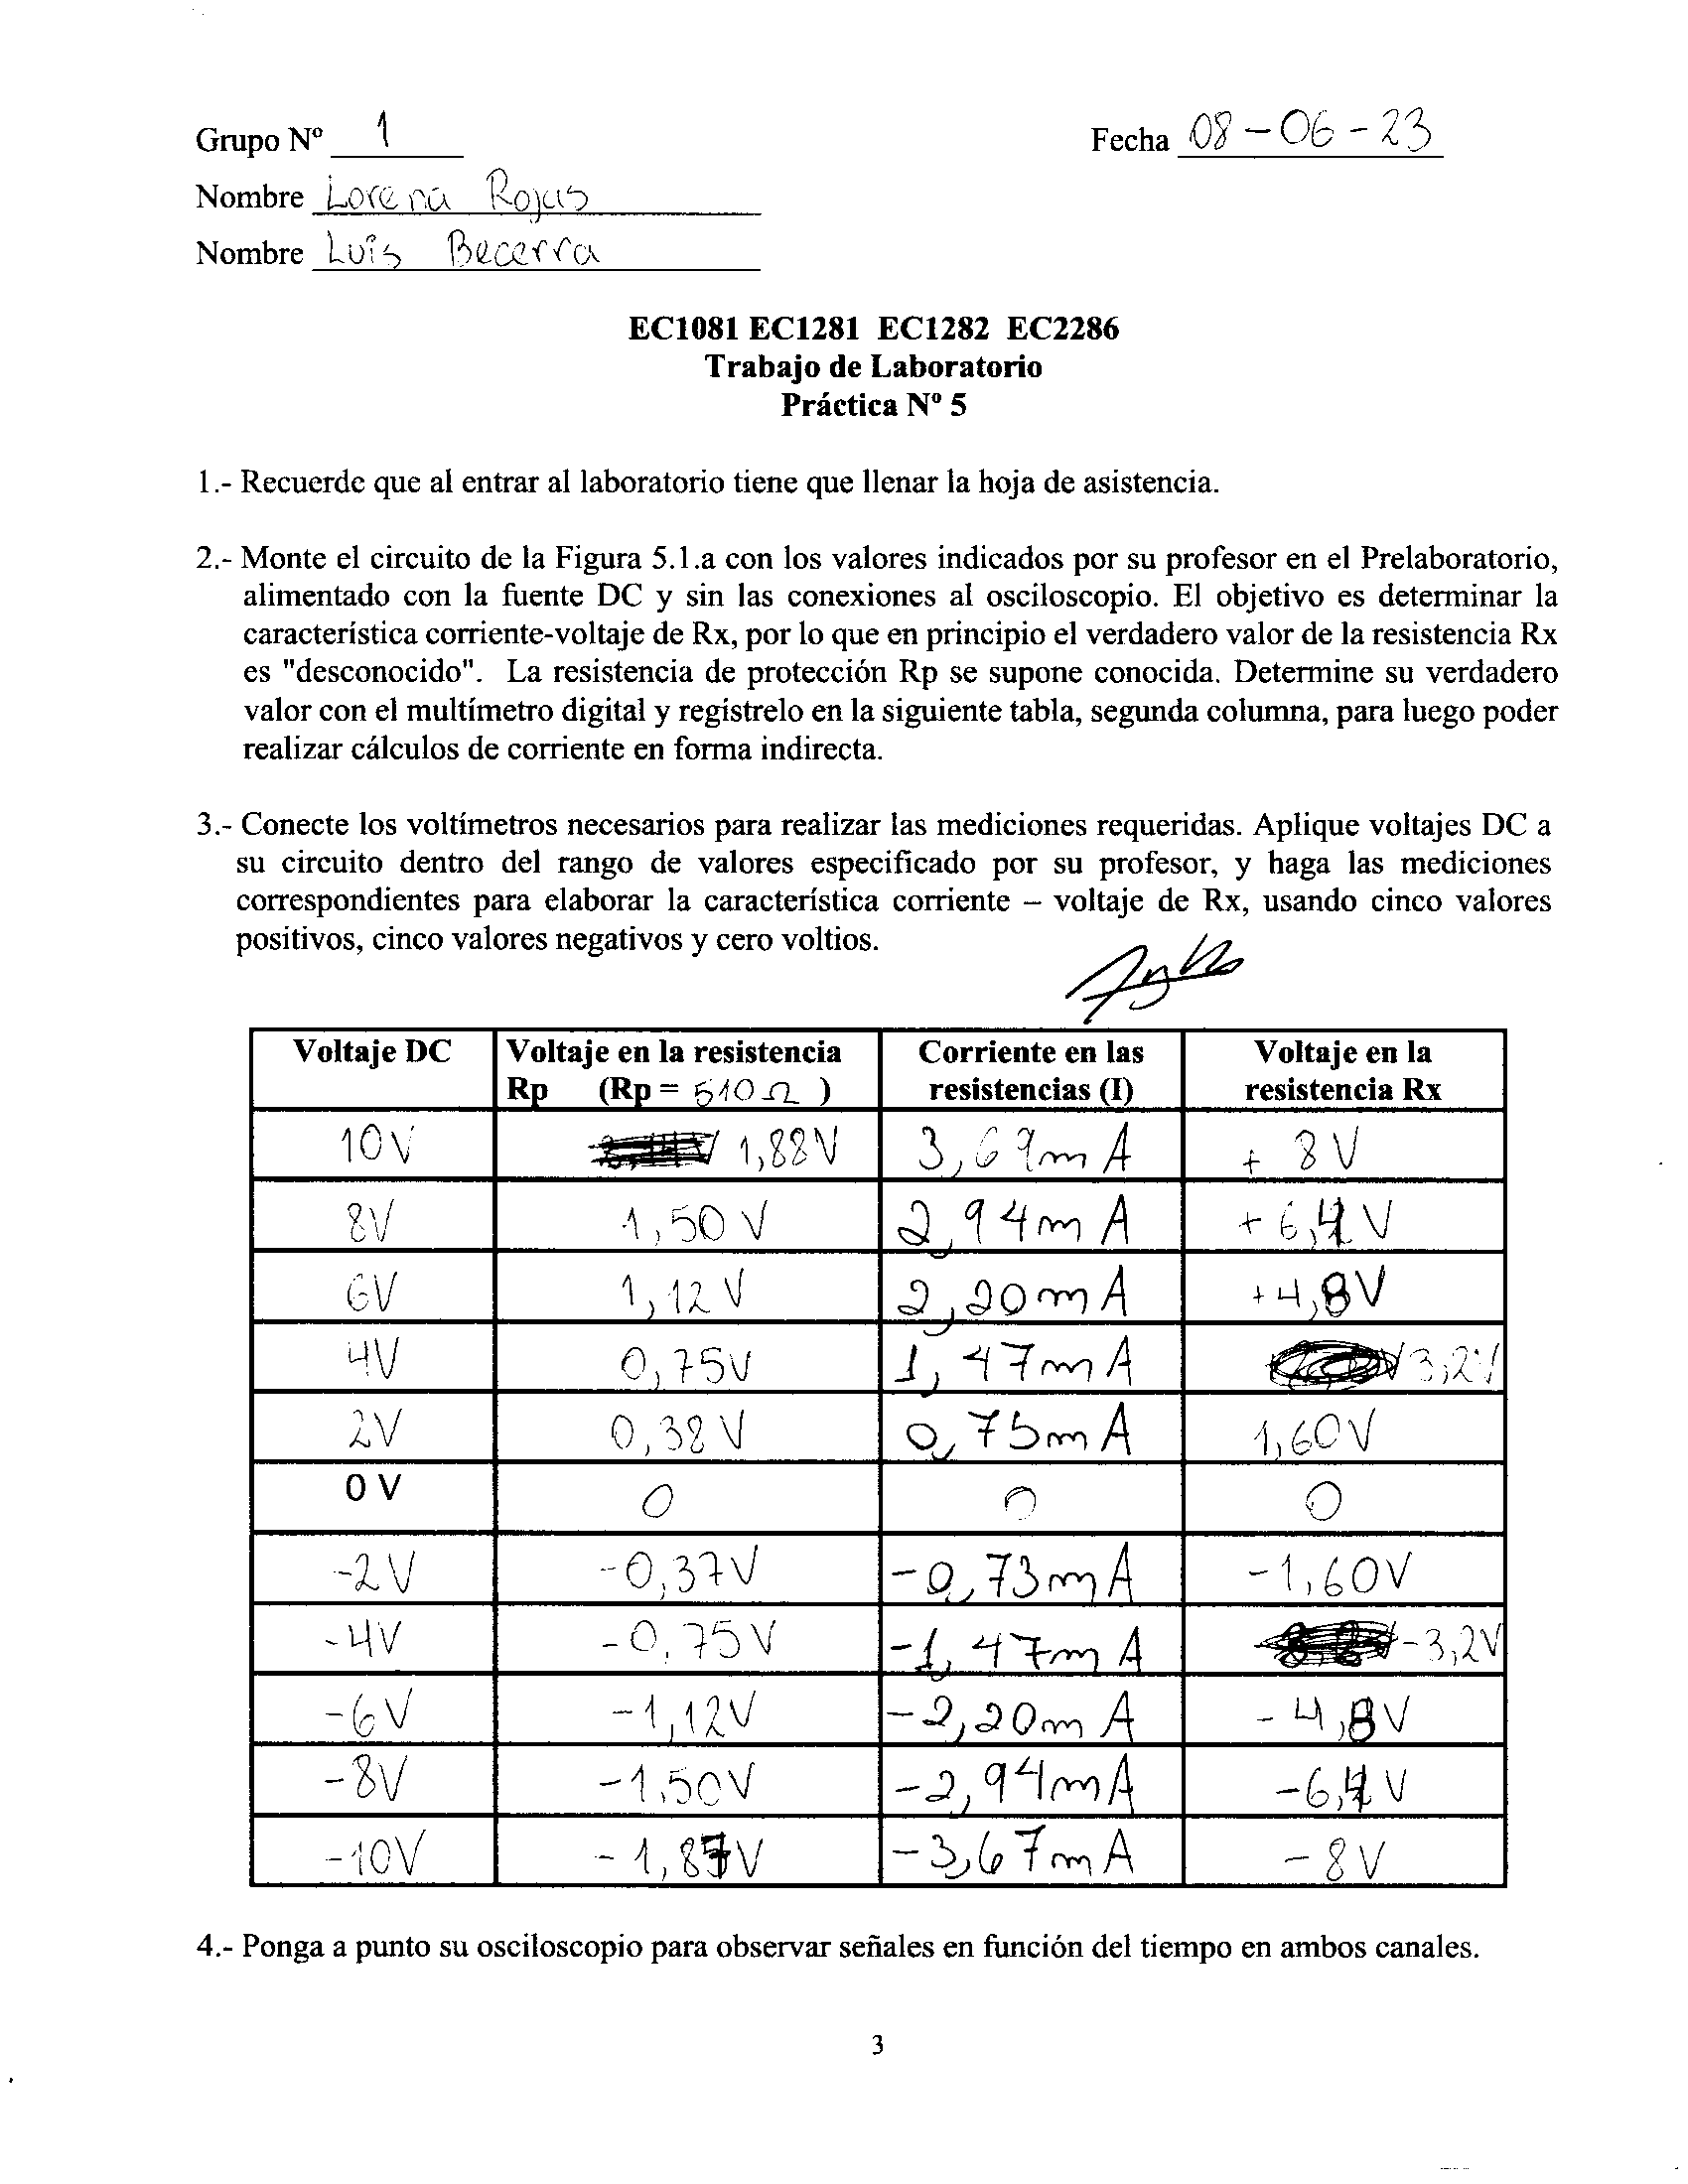
\includegraphics[width=16cm,height=20cm]{Img/anexo_0001}
	\end{center}
	
	\begin{center}
		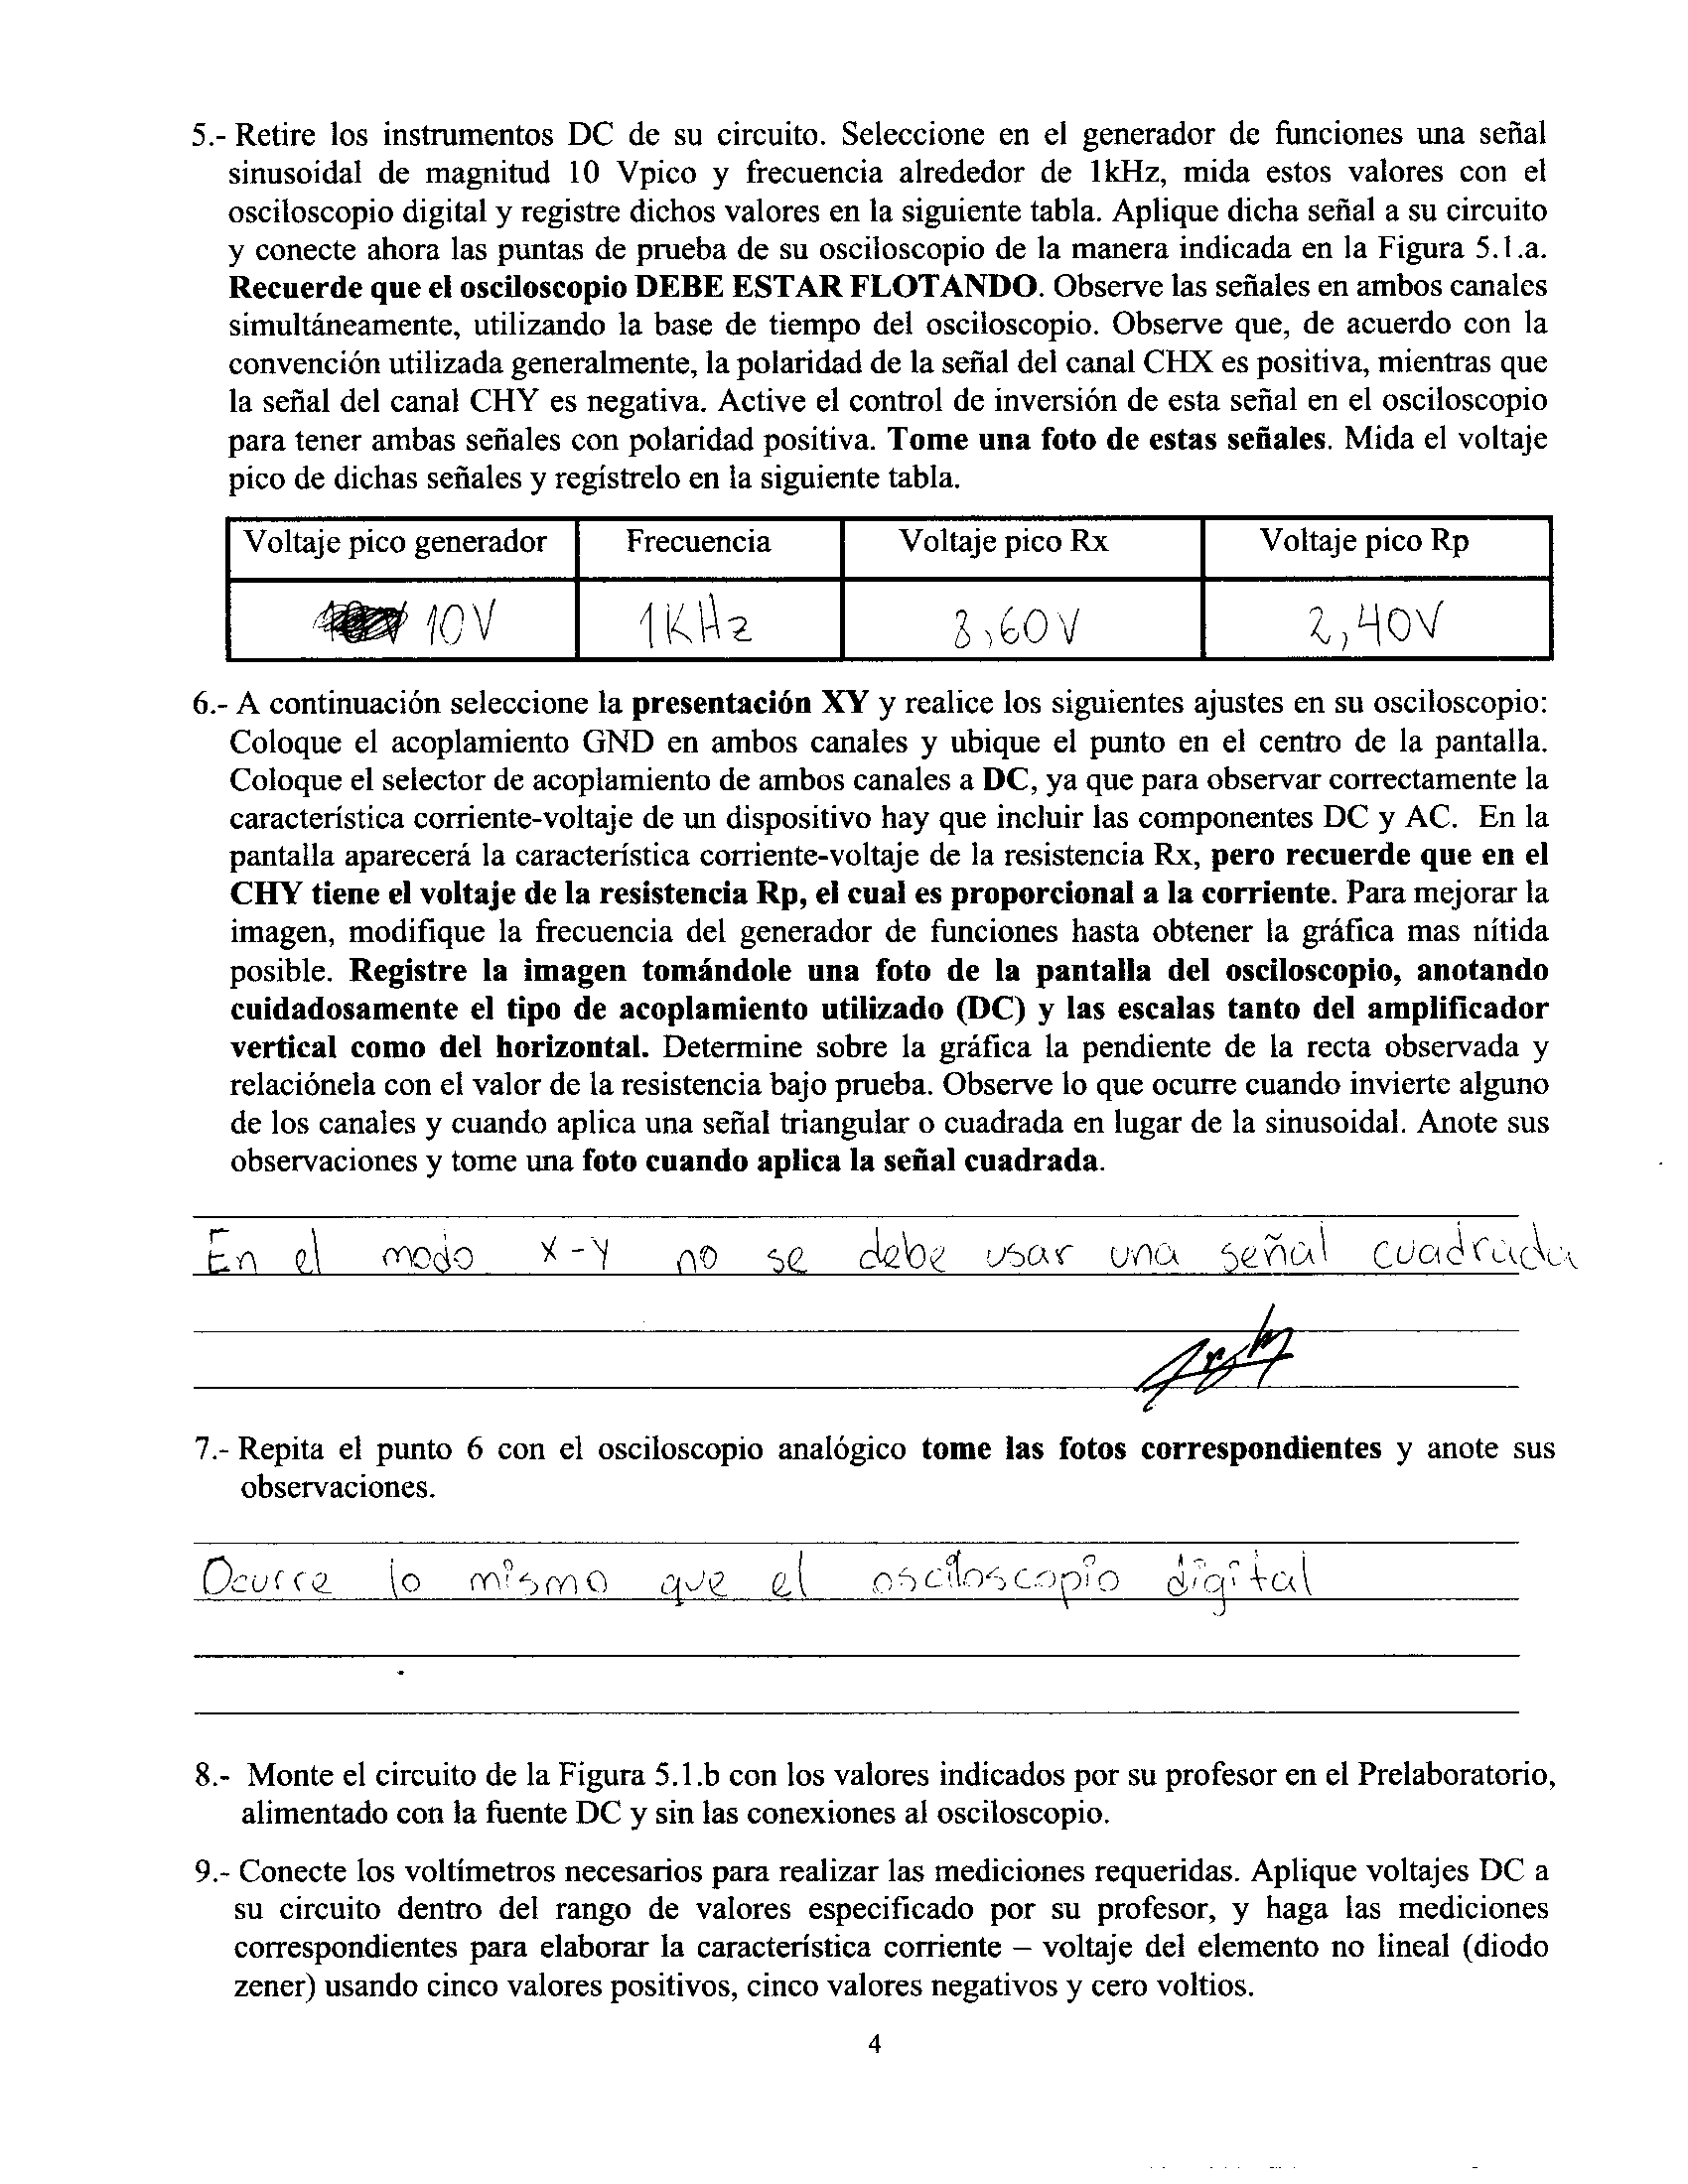
\includegraphics[width=16cm,height=20cm]{Img/anexo_0002}
	\end{center}

	\newpage
	
	\noindent Del primer circuito se tomaron las siguientes fotos del osciloscopio: 
	
	\begin{enumerate}
		
		\item Voltaje en cada resistencia modo temporal, osciloscopio digital:
		
		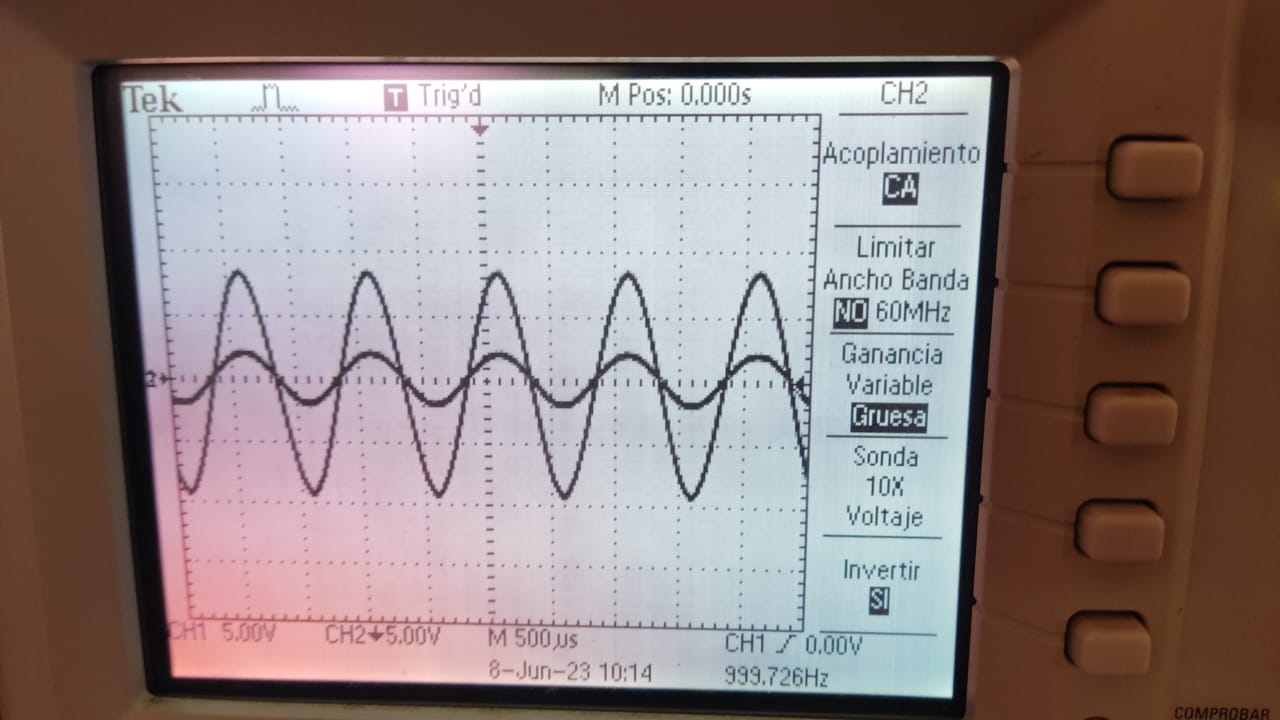
\includegraphics[width=12cm,height=7cm]{Img/lab_5_img_1}
		
		\item Voltaje en cada resistencia modo xy, osciloscopio digital:
		
		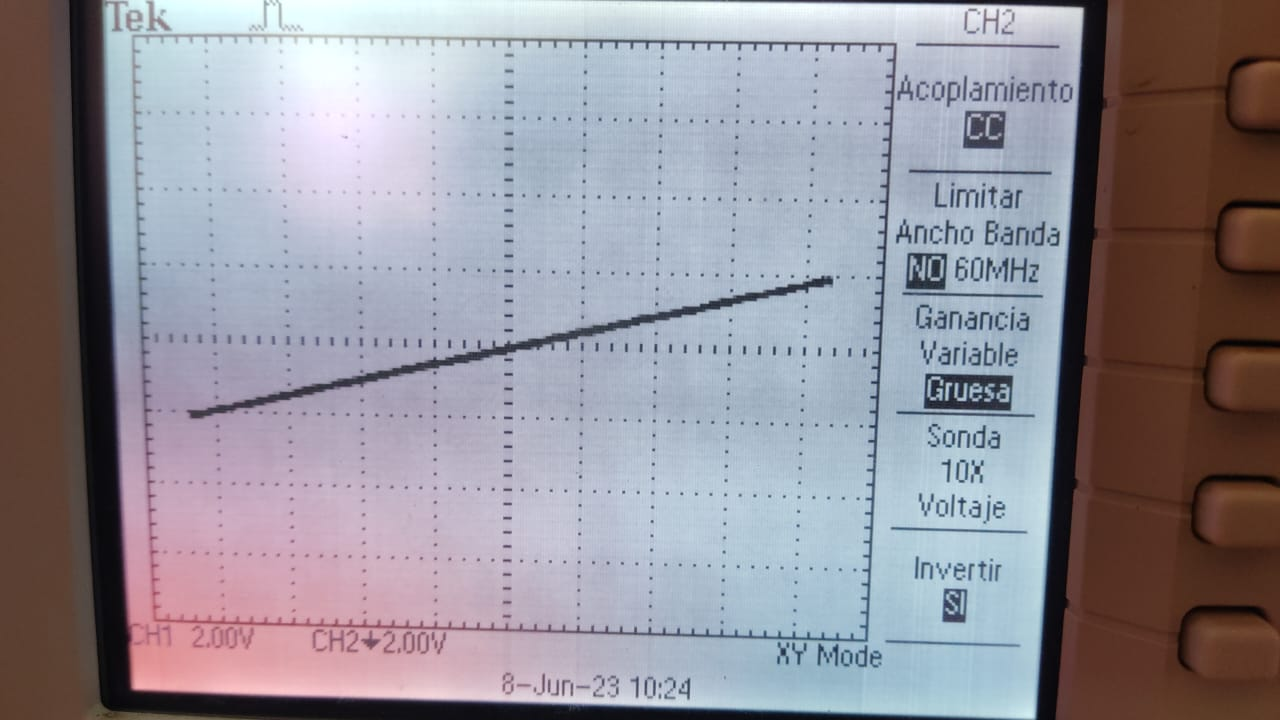
\includegraphics[width=12cm,height=7cm]{Img/lab_5_img_2}
		
		\item Voltaje en cada resistencia modo xy, onda cuadrada, osciloscopio digital:
		
		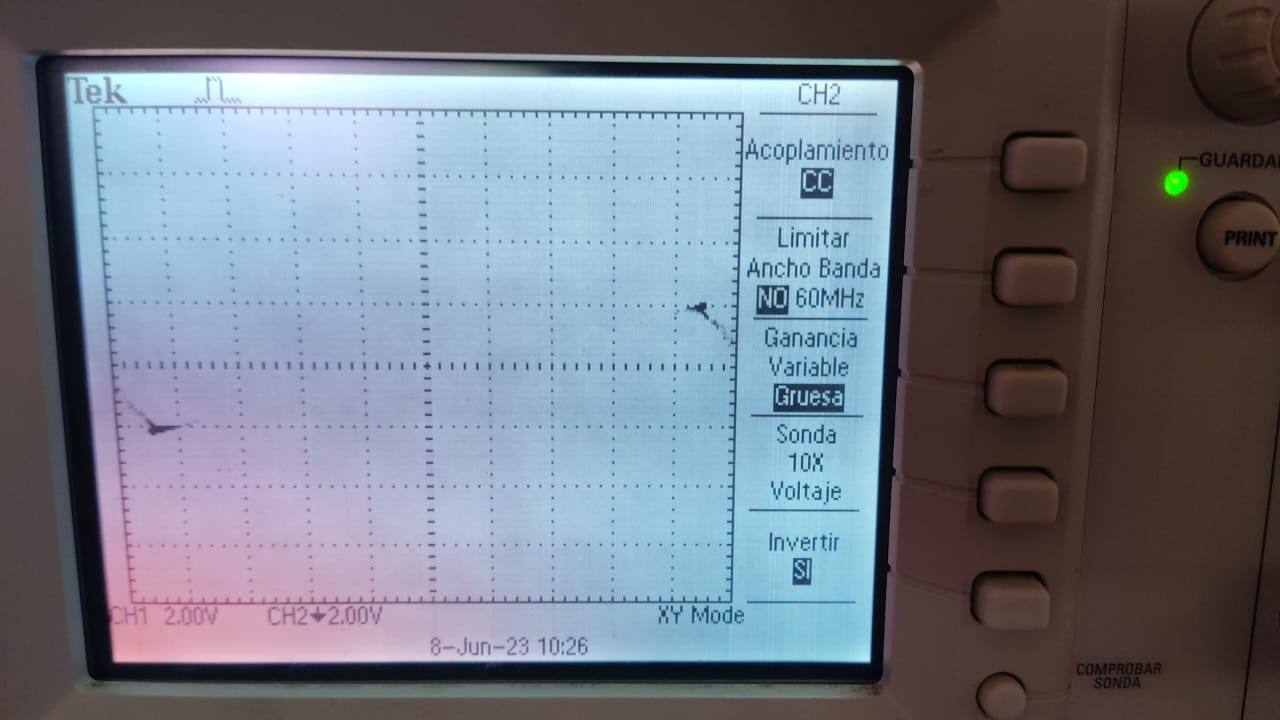
\includegraphics[width=12cm,height=7cm]{Img/lab_5_img_3}
		
		\item Voltaje en cada resistencia modo xy, osciloscopio analógico:
		
		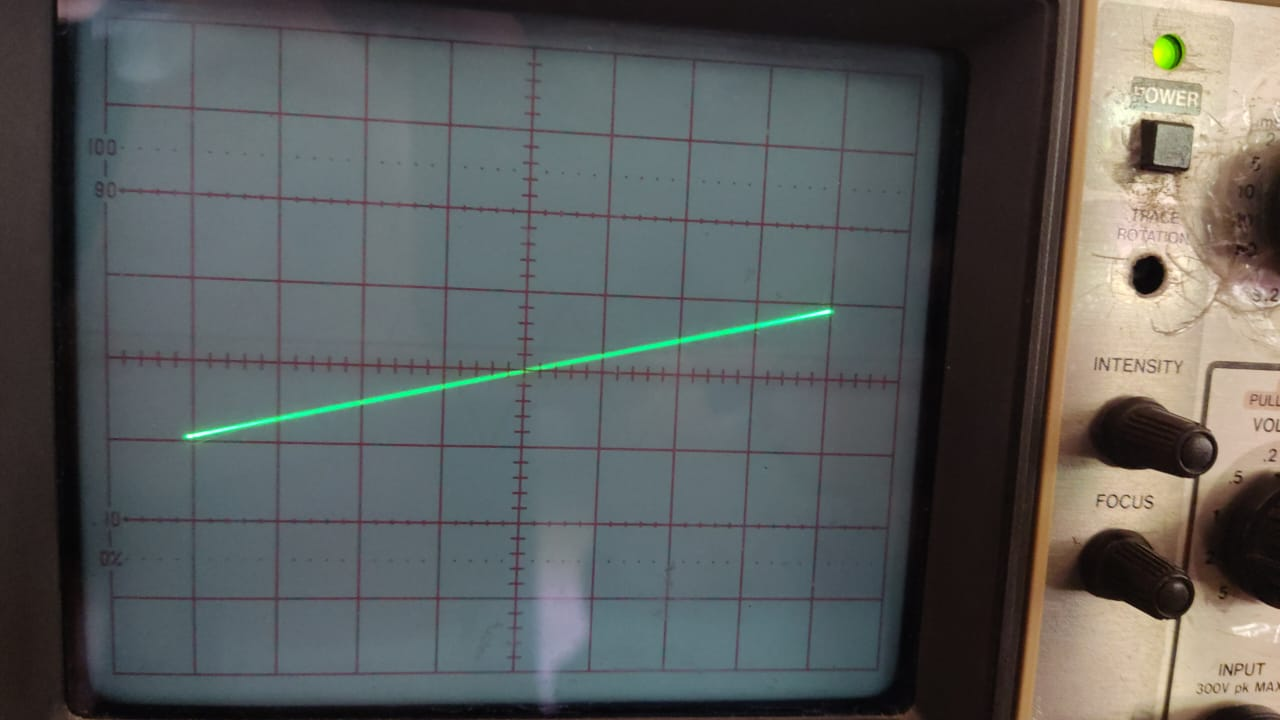
\includegraphics[width=12cm,height=7cm]{Img/lab_5_img_4}
		
		\item Voltaje en cada resistencia modo xy, onda cuadrada, osciloscopio analógico:
		 
		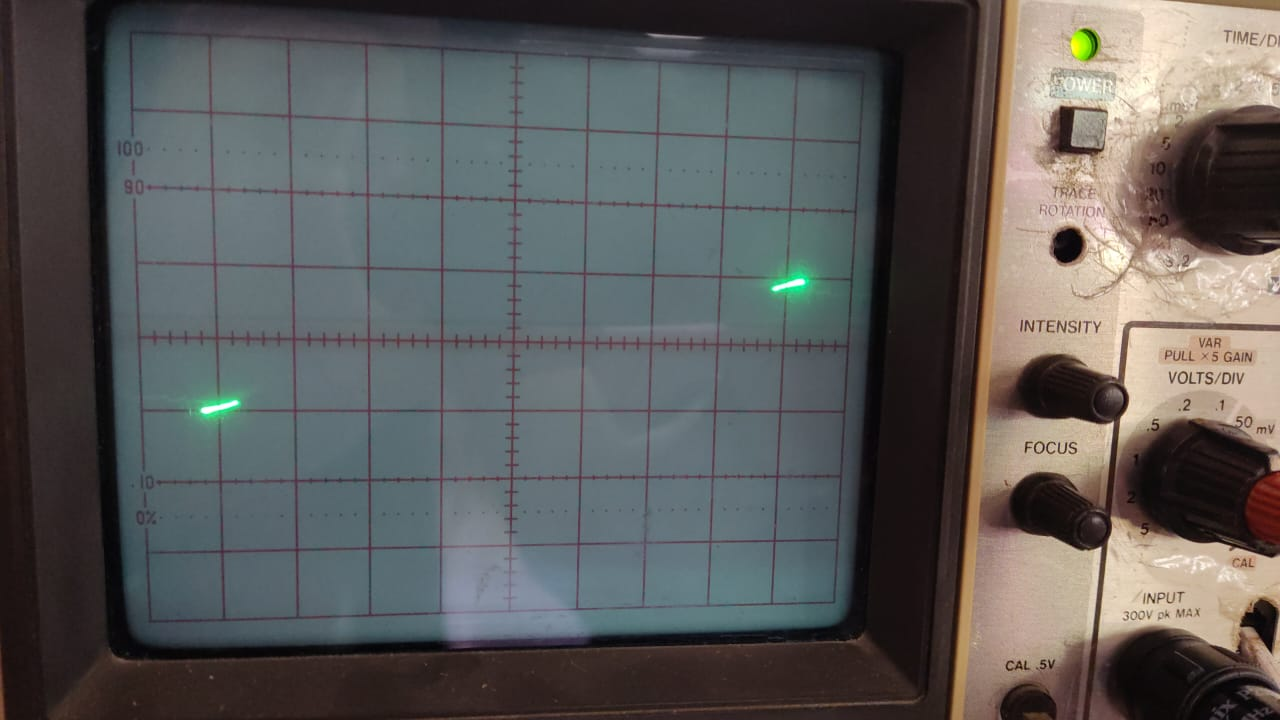
\includegraphics[width=12cm,height=7cm]{Img/lab_5_img_5}
		
	\end{enumerate}

	\newpage
	
	\begin{center}
		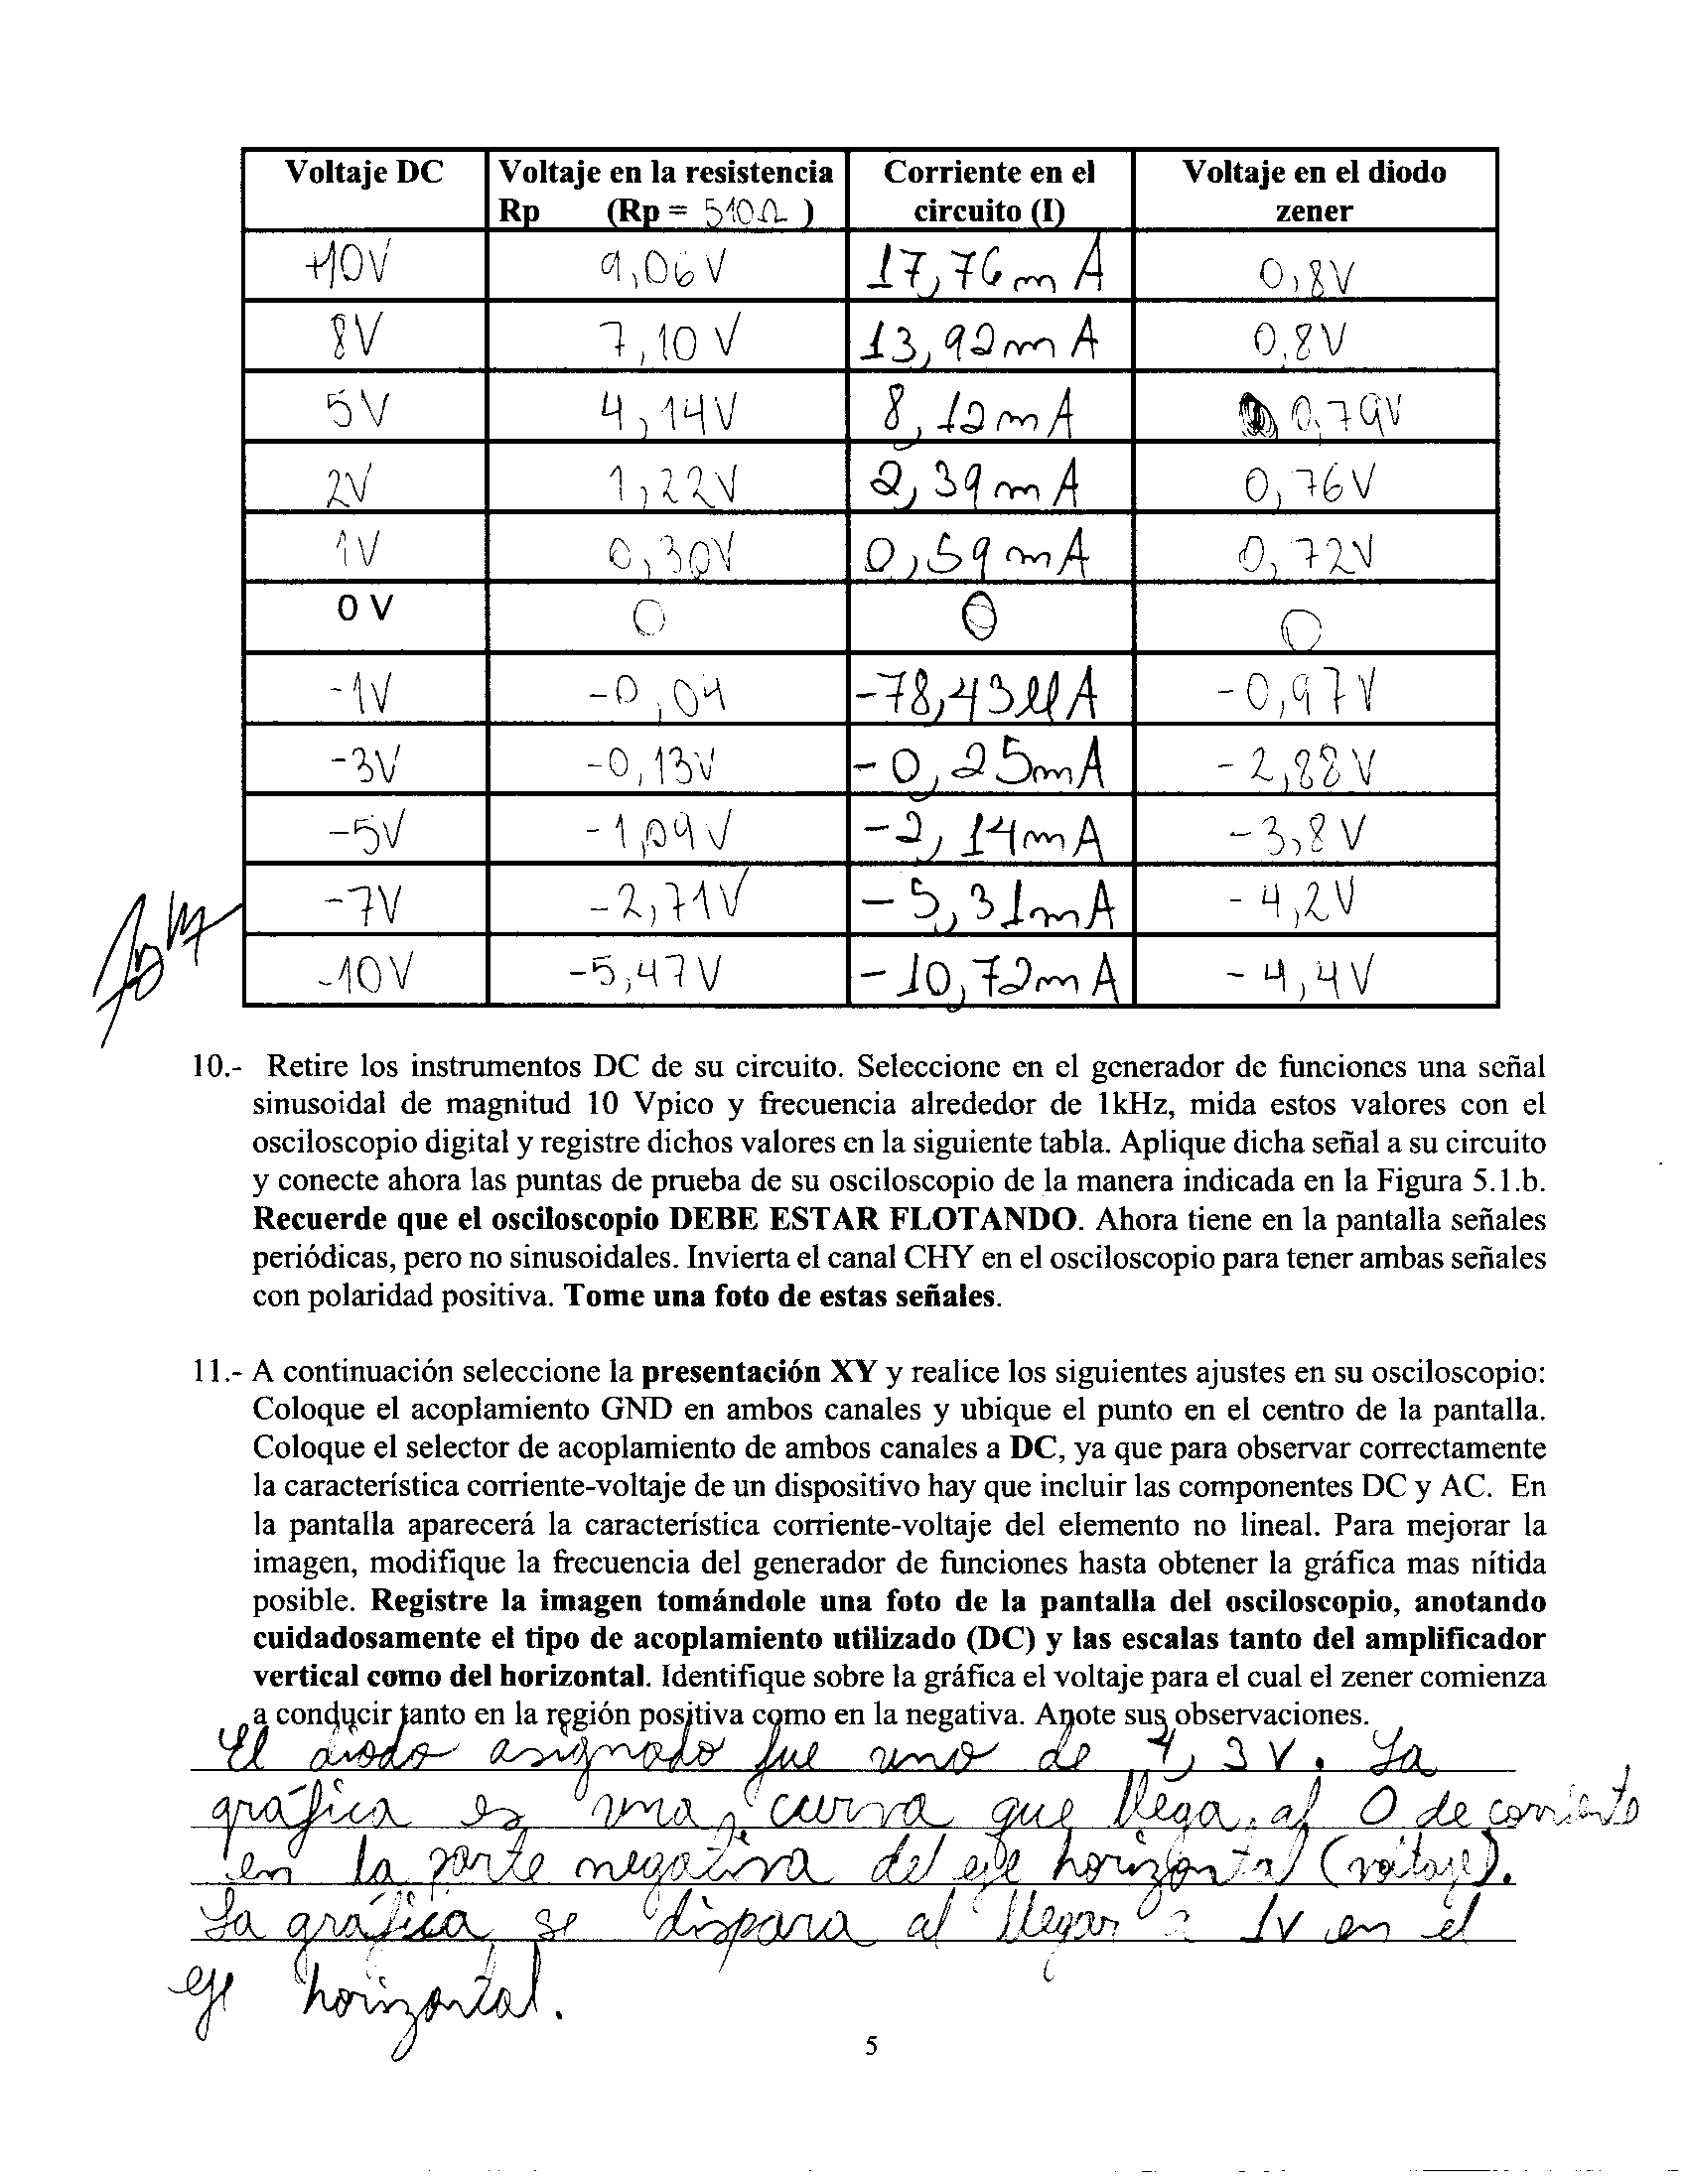
\includegraphics[width=16cm,height=20cm]{Img/anexo_0003}
	\end{center}

	\noindent Por otro lado, del circuito con el diodo se obtuvo:
	
	\begin{enumerate}
		\item Voltaje en resistencia y diodo, modo temporal:
		
		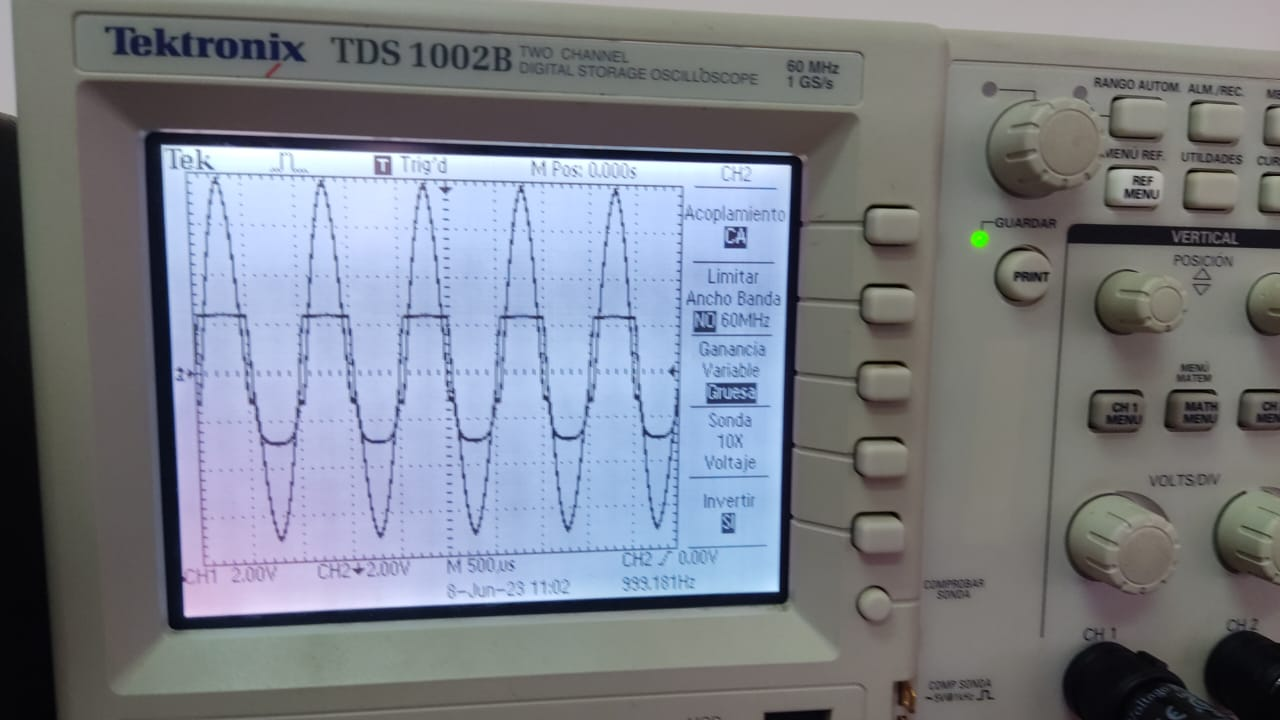
\includegraphics[width=12cm,height=7cm]{Img/lab_5_img_6}
		
		\item Voltaje en resistencia y diodo, modo xy, osciloscopio digital:
		
		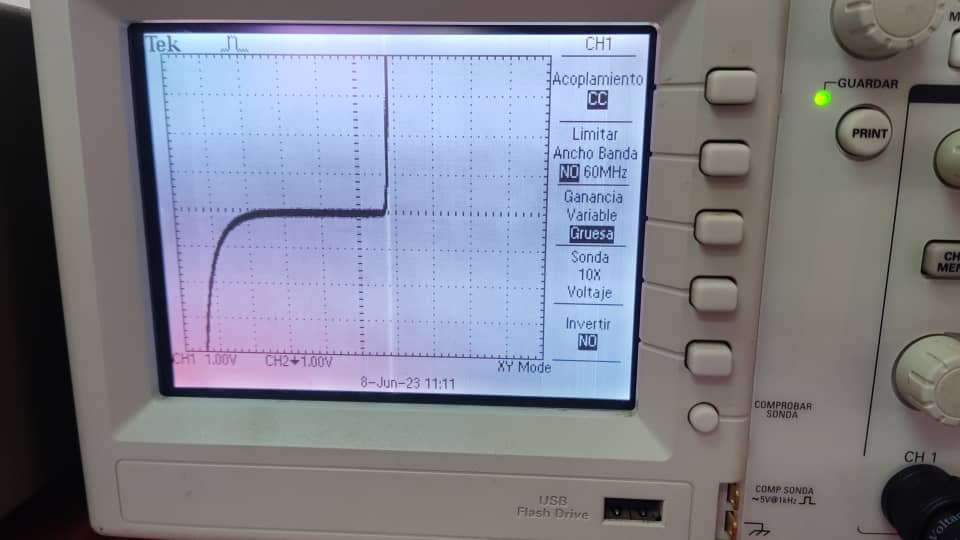
\includegraphics[width=12cm,height=7cm]{Img/lab_5_img_7}
		
		\item Voltaje en resistencia y diodo, modo xy, trazador de curvas:
		
		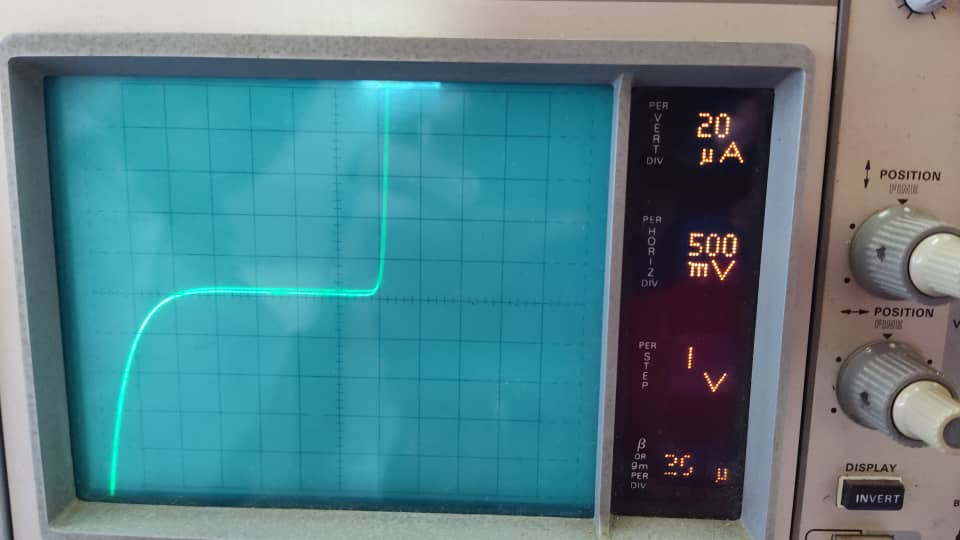
\includegraphics[width=12cm,height=7cm]{Img/lab_5_img_9}
		
		\item Voltaje en resistencia y diodo, modo xy, osciloscopio analógico:
		
		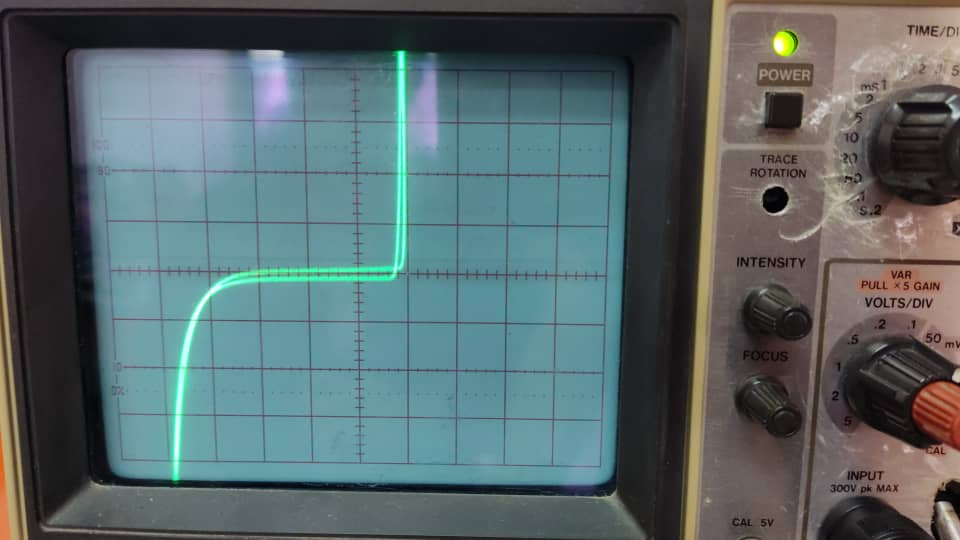
\includegraphics[width=12cm,height=7cm]{Img/lab_5_img_10}
		 
	\end{enumerate}	
	
	\begin{center}
		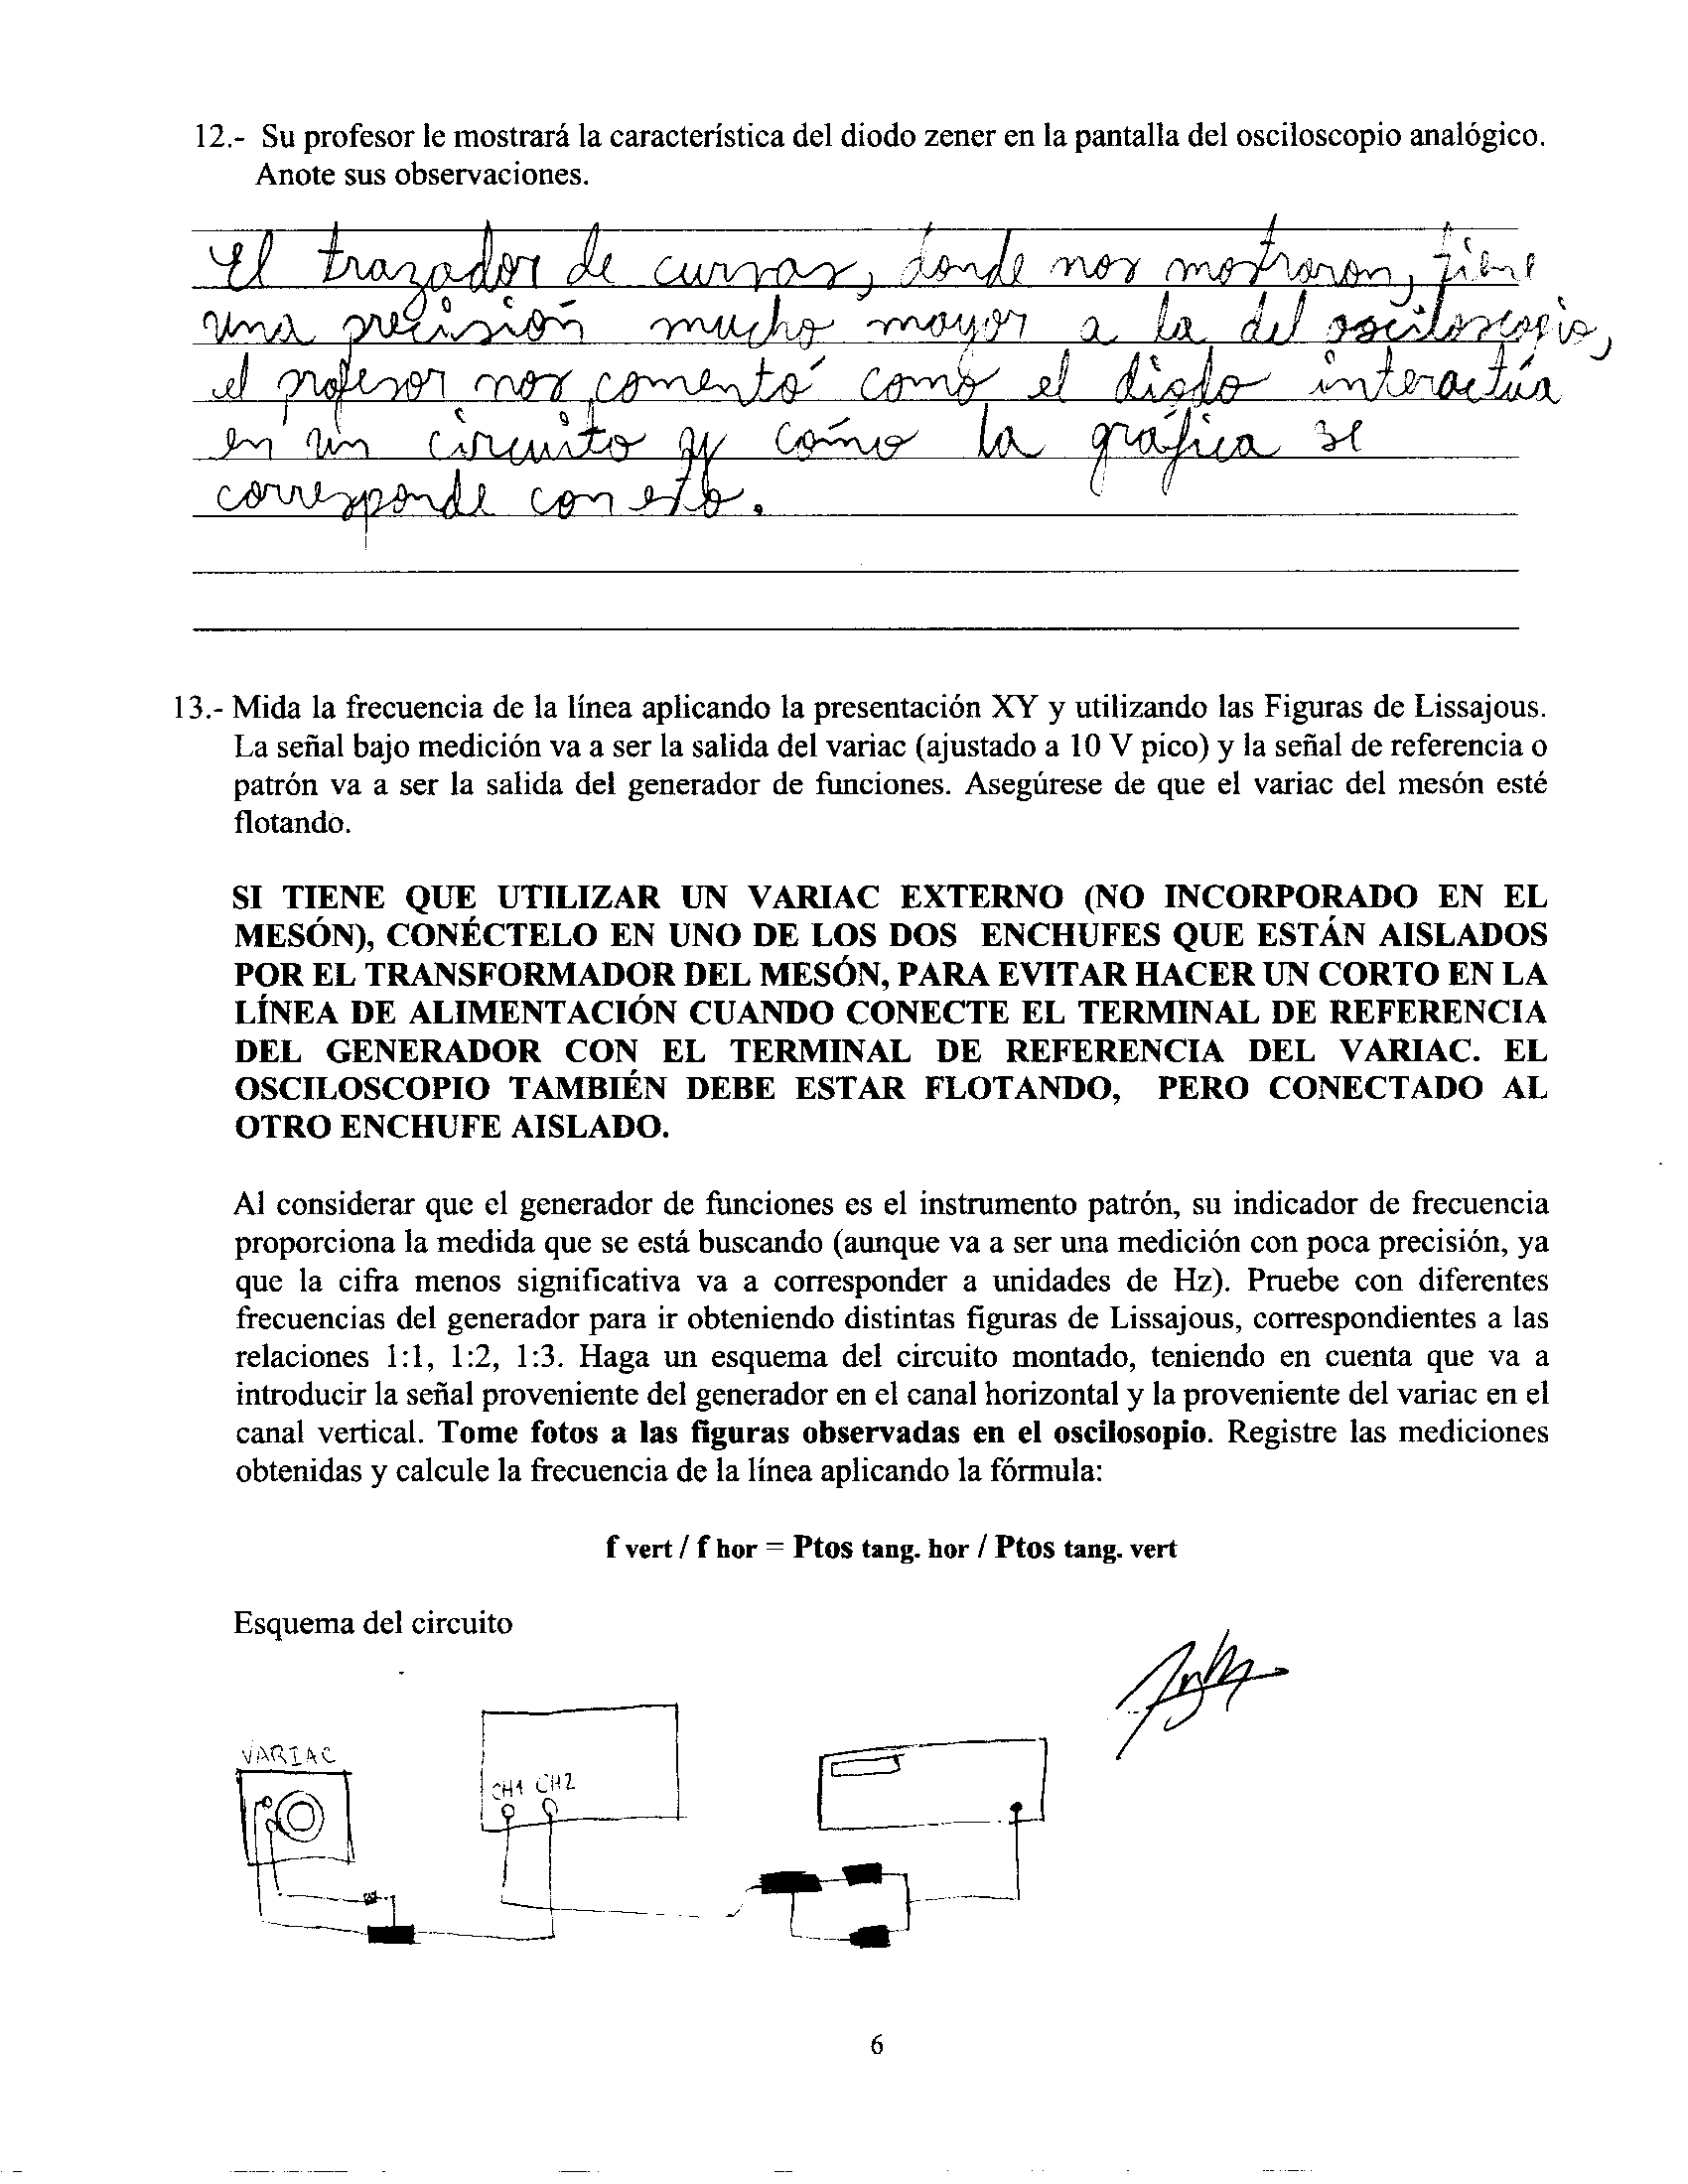
\includegraphics[width=16cm,height=20cm]{Img/anexo_0004}
	\end{center}
	
	\begin{center}
		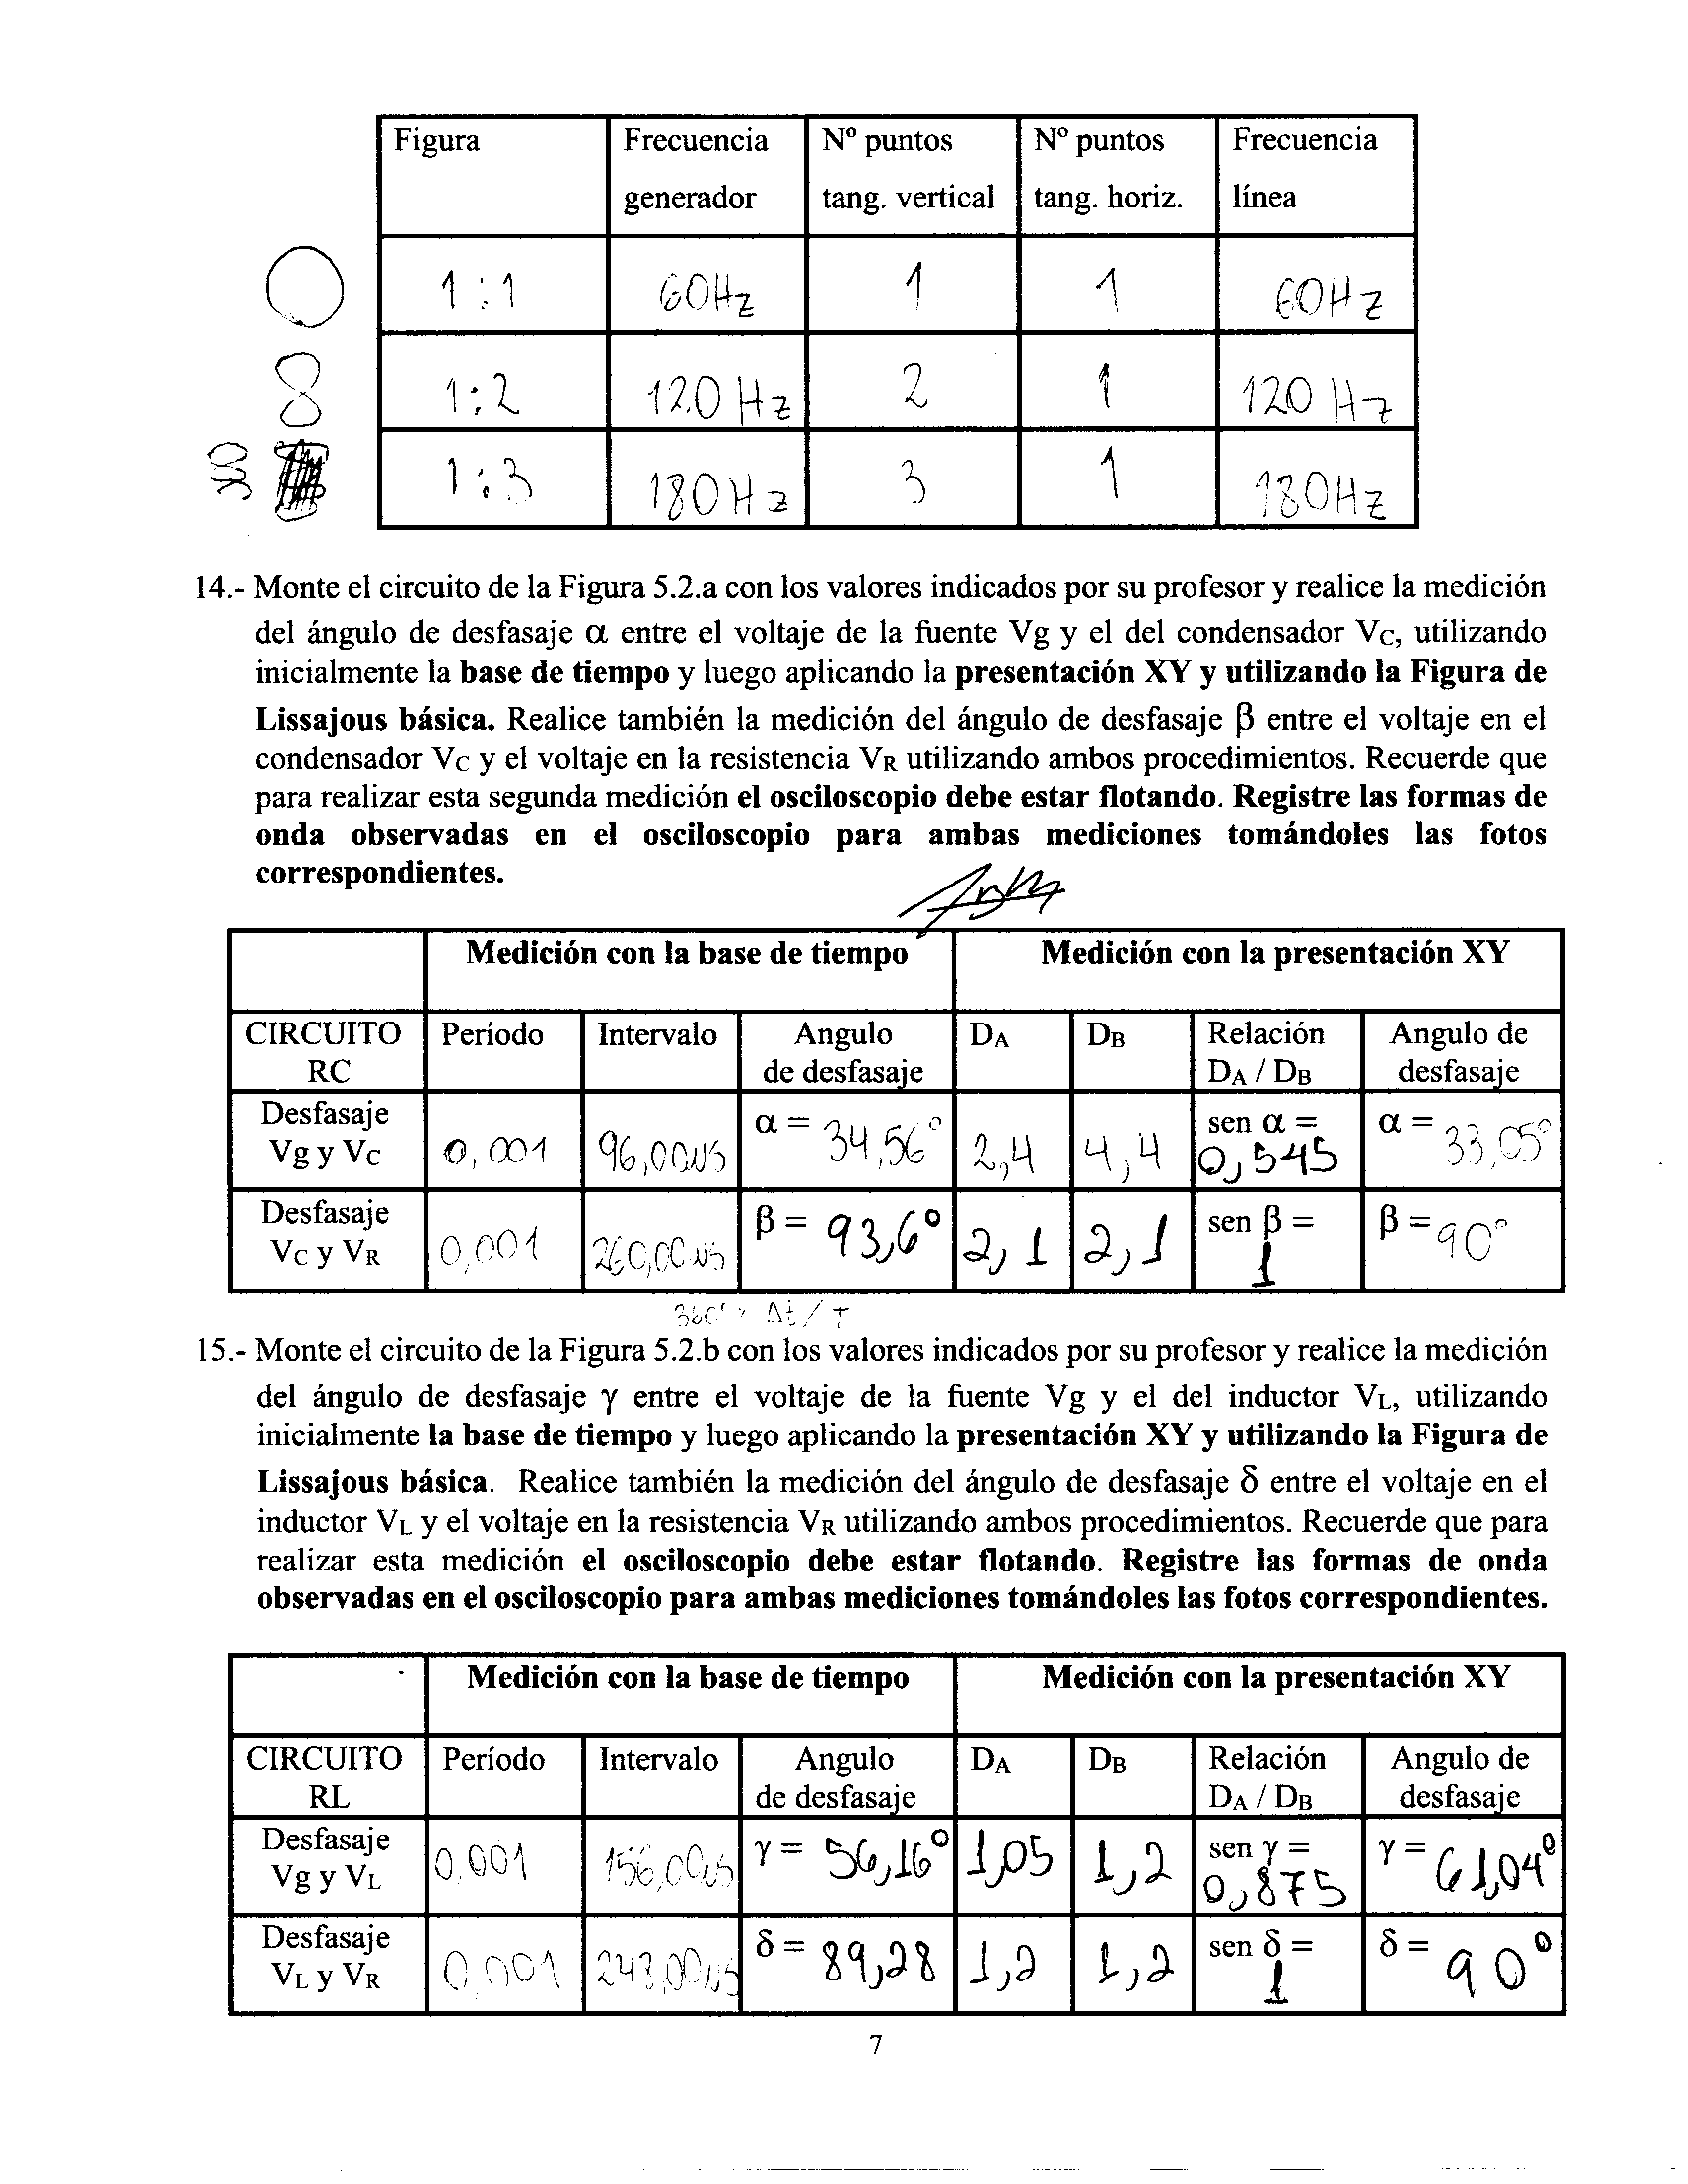
\includegraphics[width=16cm,height=20cm]{Img/anexo_0005}
	\end{center}
	
	\begin{center}
		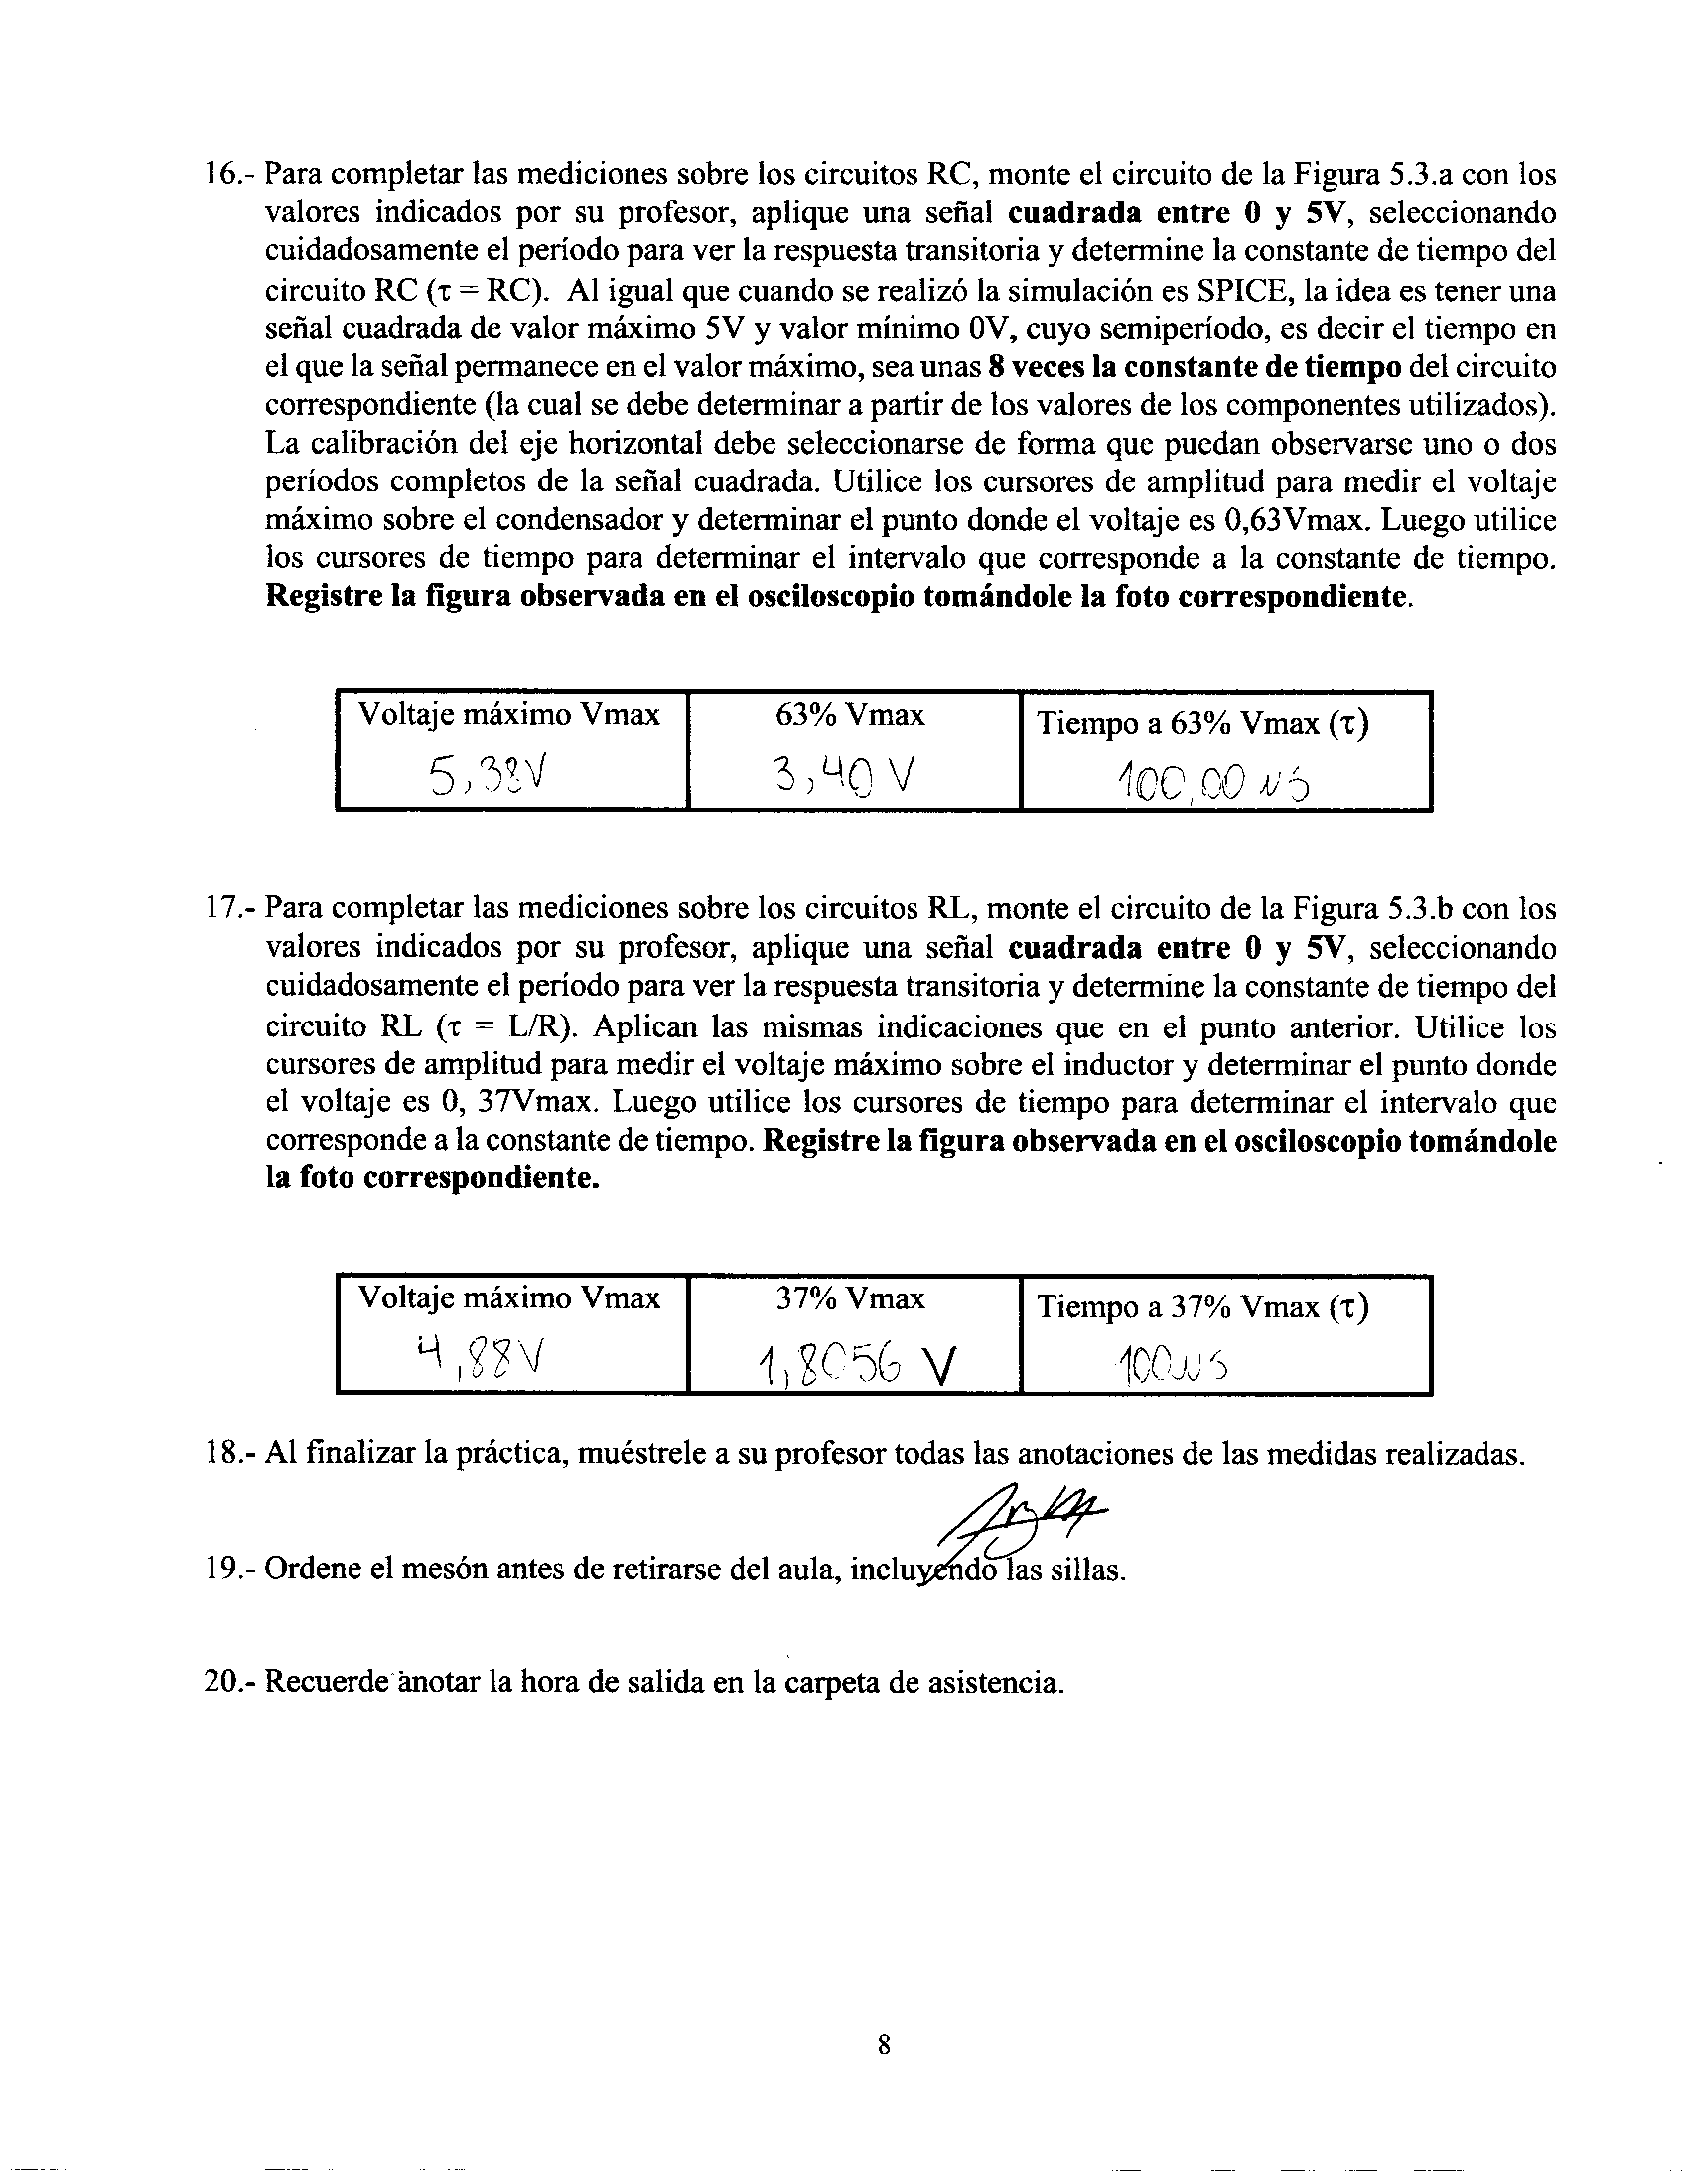
\includegraphics[width=16cm,height=20cm]{Img/anexo_0006}
	\end{center}

	\noindent Para las gráficas tendremos:
	
	
	\renewcommand{\theenumi}{\alph{enumi}} %Letras minúsculas 
	
	\begin{enumerate}
		\item Corriente vs voltaje 
	\end{enumerate}
	
	\newpage
	
	\begin{center}
		\textbf{\large ANÁLISIS DE RESULTADOS}\\
	\end{center}
	
	Inserte análisis de resultados
	
	\newpage
	
	\begin{center}
		\textbf{\large CONCLUSIONES}\\
	\end{center}
	
	Inserte conclusiones
	
	\newpage
	
	\begin{center}
		\textbf{\large BIBLIOGRAFÍA}\\
	\end{center}
	
	Inserte bibliografía
	
	\newpage
	
	\begin{center}
		\textbf{\large ANEXOS}\\
	\end{center}
	
	Inserte anexos
	
\end{document}
